\chapter{PTC power plant}
\section{Design  and simulation} \label{PTC power plant design  and simulation}
The PTC power plant was simulation in the “CSP parabolic trough (physical)" model in SAM using the option "no financial model". As before the input the EPW weather file to specify the hourly atmospheric conditions from Section~\ref{Location and weather data} was used. For the PTC simulation SAM uses the following input data:
\begin{itemize}
\item Latitude ($\,^{\circ}$)
\item Longitude ($\,^{\circ}$)
\item Elevation above sea level (m)
\item DNI (\si{\watt\per\square\metre})
\item Atmospheric pressure (\si{\milli\bar})
\item Dry bulb temperature (\si{\celsius})
\item Wetbulbtemperature(\si{\celsius})
\item Relative humidity (\si{\percent})
\item Wind velocity (\si{\metre\per\second})
\end{itemize}
This Chapter describes in detail the input data of the PTC power plant simulation by there components, namely the  power cycle, solar collector, solar receiver, solar field and thermal energy storage (TES).

Also for the simulation of the PTC are the financial parameters and the LCOE calculated separately Microfoft Excel using a simplified method which is documented in Appendix~\ref{ChapterLCOE} on Page \pageref{ChapterLCOE}.
\subsubsection{Simulated configurations}
In order to reaching the goal of covering 90 \% of the scheduled production curve also the simulated PTC power plant used a variation of solar multiple and full load hours of TES. To covering the scheduled load the solar multiple was varied from 2 to 5.0 in steps of 5.0. This is significantly higher SM compared the simulated CR system was necessary to reach the \SI{90}{\percent} covering factor. As before with the simulation of the CR, the storage full load hours were varied from \si{8} to \SI{16}{h} in steps of \SI{2}{h}. The target of \SI{100}{MW} net capacity was reached with a gross capacity of \SI{120}{MW} with an estimated gross-to-net conversion factor of \si{0.83}. The comparatively high gross turbine output is nessasary for the high parasitic burden of the system. Table~\ref{tbl: PTC_OverallConfig} summarizes the simulated configurations.
\begin{table}[!h]  
  \centering
	\begin{tabular}{ p{4.0cm}  C{1.0cm}  C{0.3cm} C{0.3cm} C{0.3cm} C{0.3cm} C{0.3cm} |C{0.3cm}  C{0.3cm} C{0.3cm} C{0.3cm} C{0.3cm} } 
	\hline	
\textbf{Item} & \textbf{Unit} & \multicolumn{10}{c}{\textbf{Value}} \\ \hline \hline
Net turbine capacity & \si{\mega\wattel} & \multicolumn{10}{c}{100} \\
Gross turbine capacity & \si{\mega\wattel} & \multicolumn{10}{c}{120} \\ \hline
Solar multiple & - & \multicolumn{5}{c}{2.0} & \multicolumn{5}{c}{2.5} \\
TES capacity & h & 8 & 10 & 12 & 14 & 16 & 8 & 10 & 12 & 14 & 16 \\ \hline 
Solar multiple & - & \multicolumn{5}{c}{3.0} & \multicolumn{5}{c}{3.5} \\
TES capacity& h & 8 & 10 & 12 & 14 & 16 & 8 & 10 & 12 & 14 & 16 \\ \hline 
Solar multiple & - & \multicolumn{5}{c}{4.0} & \multicolumn{5}{c}{4.5} \\
TES capacity& h & 8 & 10 & 12 & 14 & 16 & 8 & 10 & 12 & 14 & 16 \\ \hline 
Solar multiple & - & \multicolumn{5}{c}{5.0} & \multicolumn{5}{c}{ } \\
TES capacity& h & 8 & 10 & 12 & 14 & 16 &  \multicolumn{5}{c}{ } \\ \hline 
\end{tabular}
\caption[Simulated PTC solar multiple and thermal energy storage  configurations.]{Simulated PTC solar multiple and thermal energy storage  configurations.}\label{tbl: PTC_OverallConfig}
\end{table}

\subsubsection{Power cycle}
The PTC system also uses the steam Rankine cycle technology. In the modeled cycle, feedwater is heated in open (mixed stream) feedwater heaters with two intermediate turbine extractions - once for high pressure and once for low pressure, and the steam generation equipment consists of a preheater, boiler, and superheater. The HTF temperature at the field outlet is bound primarily by HTF stability, so maximum HTF temperatures for oil troughs typically range between \SI{370}{\celsius} and \SI{410}{\celsius}. The turbine has a gross capacity of \SI{120}{\mega\wattel}. So the net turbine capacity output at design (nameplate) is \SI{100}{\mega\wattel}. The design inlet temperature of the HTF in the steam generator is 393\si{\celsius} and outlet temperature of 293\si{\celsius} at design point and operates at a pressure of 100 bar.



Table~\ref{tbl: PTCPowerplant} shows the input parameter for the power block design in SAM. Besides the capacity of the turbine and the condecer type, the parameters are coming from \cite{Wagner2011}. It is obviously, that the cycle conversion efficiency of the PTC power plant is lower than that one from the CR power plant. This is trace back to the lower cycle temperatures and the thereby resulting lower steam pressure in the turbine.



The air-cooled condenser was selected here as well, because water is an valuable resource in the region of Upington. The cooling system is designed to covers the stem generator thermal power. 
\begin{table}[!h]  
  \centering
	\begin{tabular}{  p{7.0cm}  C{2.0cm}  C{2.0cm} } 
	\hline	
\textbf{Item} & \textbf{Value} & \textbf{Unit} \\ \hline \hline
Turbine design capacity, gross  & 110 & \si{\mega\wattel} \\ 
Turbine design capacity, net & 100 & \si{\mega\wattel} \\ 
Boiler operating pressure & 100 & bar \\ 
Design inlet temperature & 393 & \si{\celsius} \\ 
Design outlet temperature & 291 & \si{\celsius} \\ 
Cycle conversion efficiency & 37.74 & \% \\ 
Steam generator design thermal power & 318.0 & \si{\mega\wattth}  \\
Power block start-up time & 0.5 & h \\ 
Minimum required start-up temperature & 300 & \si{\celsius} \\
Maximum turbine over design operation & 90 & \\
Condenser type & air-cooled & - \\ 
\hline
\end{tabular}
\caption[PTC power block and condecer input parameter in SAM.]{PTC power block and condecer input parameter in SAM.}\label{tbl: PTCPowerplant}
\end{table}
\subsubsection{Solar collector (SCA)}
For the simulation of the PTC system the Ultimate Trough was selected as solar collector assembly (SCA). This collector is currently not in commercial use, but comparable troughs with similar characteristics are under construction. So the Ultimate Trough can be adopted  without technical modifications and no increase of risk. Figure~\ref{PTC_Ultimate_config} shows the information of the technical input parameter for SAM. These coming directly from a publication of the developer of the Ultimate Trough, Flabeg GmbH and sbp sonne GmbH \cite{Riffelmann2014}. 
\begin{figure}[bhtp]
\centering
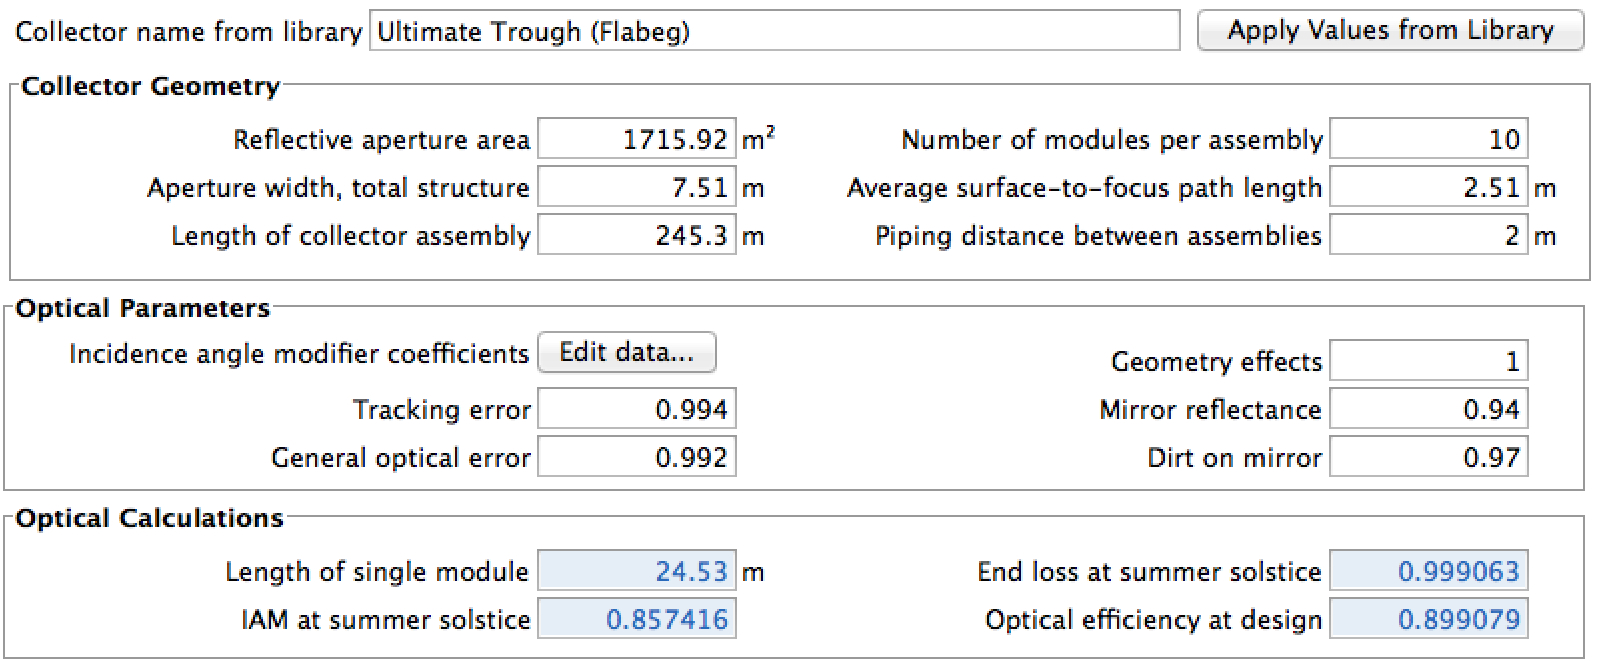
\includegraphics[width=0.95\linewidth]{FIG/PTC_Ultimate_config}
\caption[Screenshot of Ultimate Trough SCA input parameter for SAM.]{Screenshot of Ultimate Trough SCA input parameter for SAM.}\label{PTC_Ultimate_config}
\end{figure}
The section "Optical Calculation" shows, that the total optical efficiency at design of the Ultimate Trough is 89.9~\%. The dimensions and main characteristics of the HCE is shown in the section "Receiver Geometry".
\subsubsection{Solar receiver (HCE)}
As heat collecting element (HCE) Schott's PTR80 was selected. This receiver tube has with \SI{0.08}{m} an extended tube outer diameter. Thereby the tube can contain more HTF and reduce the mass flow in the tubes. Figure~\ref{PTC_HCE} shows the for the simulation inserted parameter. The values are the results of measurements of outdoor optical efficiency and indoor receiver heat loss of parabolic trough collector from researchers of the American National Renewable Energy Laboratory \cite{Kutscher2012}.
\begin{figure}[htbp]  
\centering
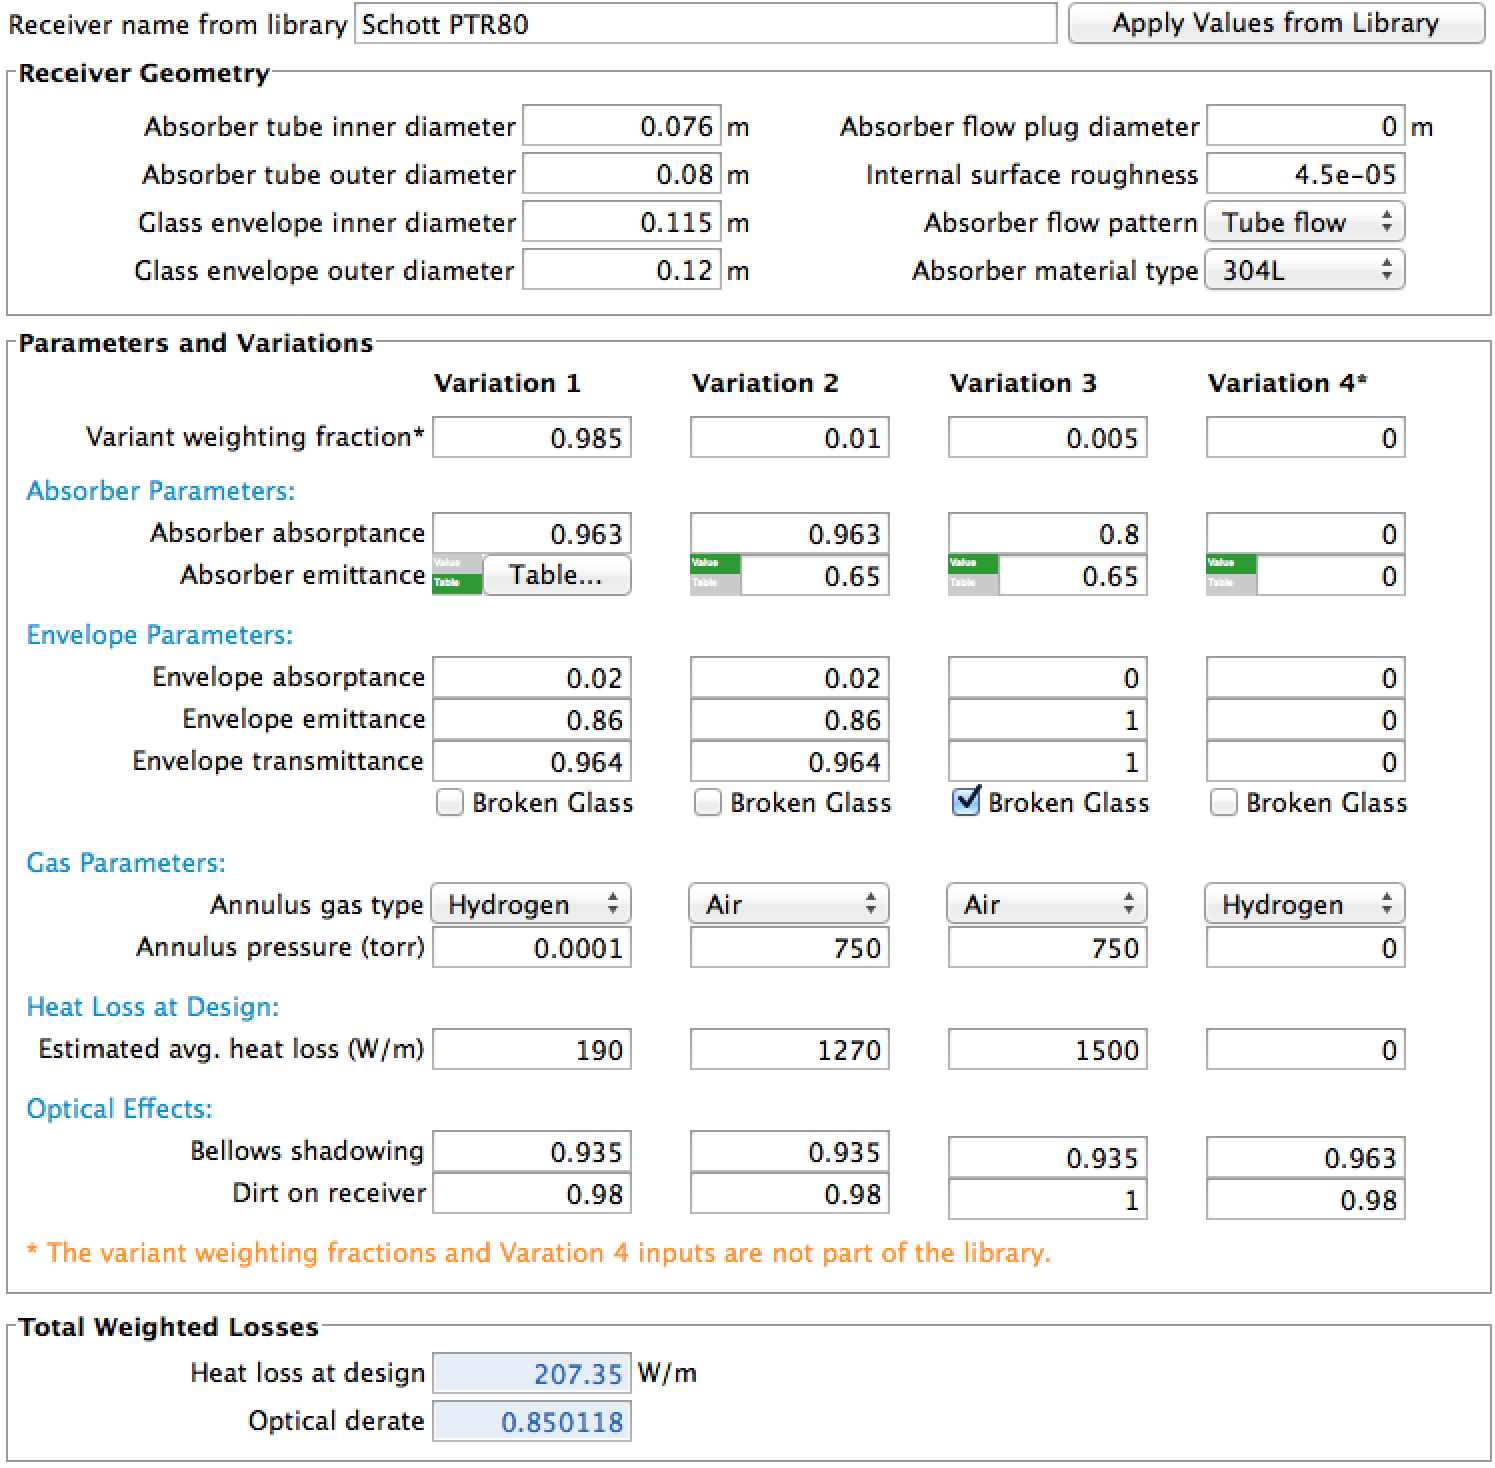
\includegraphics[width=0.95\linewidth]{FIG/PTC_HCE}
\caption[Screenshot of Schott PTR80 input parameter for SAM.]{Screenshot of Schott PTR80 input parameter for SAM.}\label{PTC_HCE}
\end{figure}
The section "Parameter and Variations" shows the different conditions of the HCE. Variation 1 shows the optimal condition of the HCE with annulus pressure of 0.0001 torr (\SI{0.000133}{hPa}), so an vacuum. The estimated average heat lost is \SI{190}{W/m}. This Variation counts for 98.5~\% of all HCEs. In Variation 2 the vacuum is lost and which strongly affects the heat loss. It is 1~\SI{270}{W/m} and counts for 1~\% of all HCEs. In Variation 3 also the protection glass is broken, so the heat loss increase to 1~\SI{500}{W/m}. The total weighted losses is \SI{207.35}{W/m} heat loss at design and about 0.85 optical derate and is shown at the last section most below.
\subsubsection{Solar field}
PTC solar fields are separated in sections. In the simulation of the PTC system the solar field is designed in two sections. Each section carries a feed pipe and a return pipe to transport the thermal energy to the power block. Attached to the header pipes are many loops, which contains the SCAs, the HCEs and the HTF. Figure~\ref{PTC_Field_ultimate} shows an typical layout for PTC system with two field subsections. As in the Figure is the simulated PTC system designed by four SCAs per loop \cite{Riffelmann2014}.
\begin{figure}[htbp]  
\centering
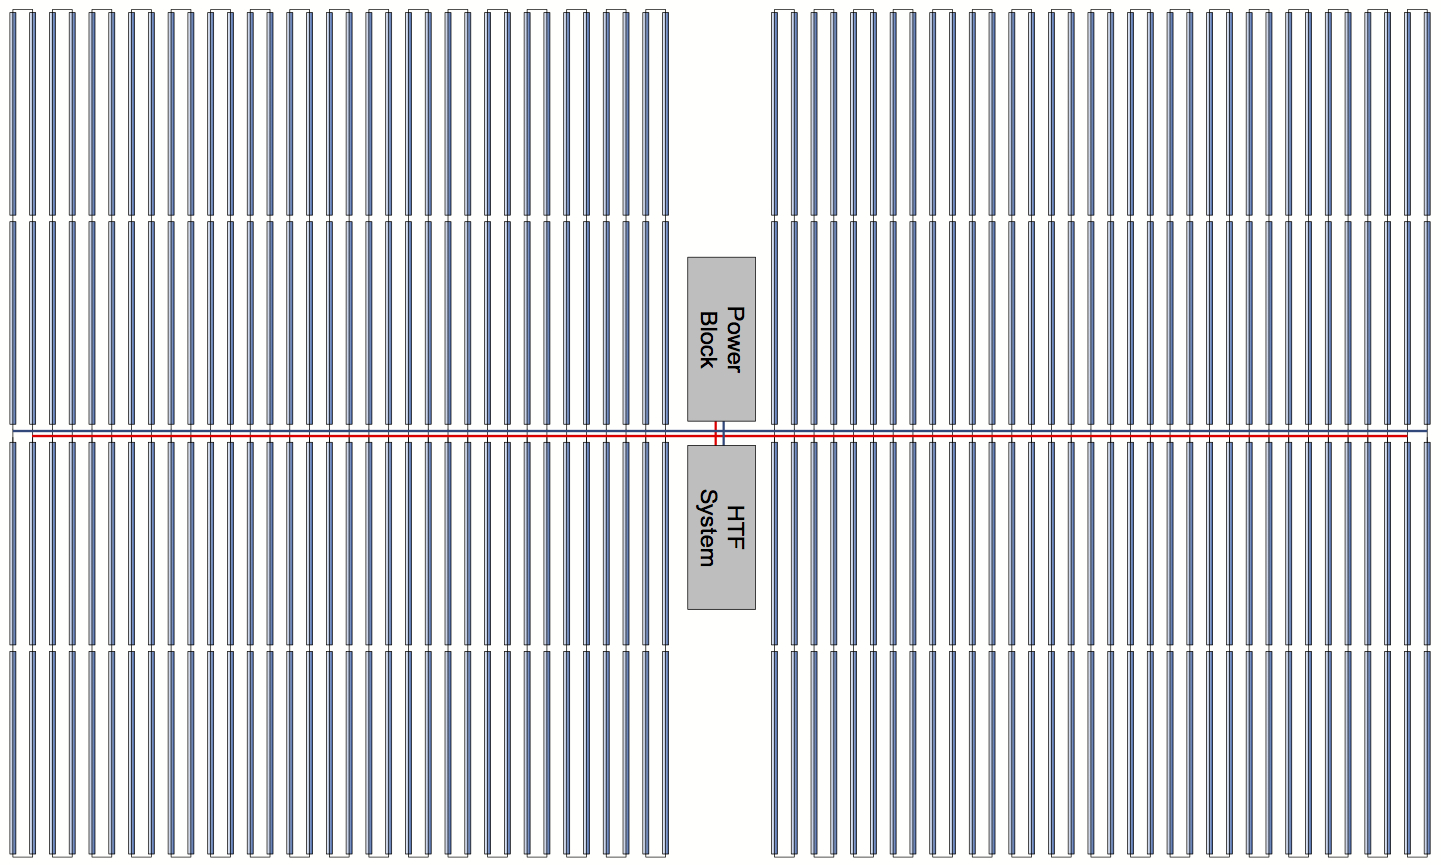
\includegraphics[width=0.9\linewidth]{FIG/PTC_Field_ultimate}
\caption[Typical configuration of a solar field layout with two field subsections for a Ultimate Trough.]{Typical configuration of a solar field layout with two field subsections for a Ultimate Trough \cite{Riffelmann2014}.}\label{PTC_Field_ultimate}
\end{figure}


As mentioned before synthetic oil is used as HTF for the simulation of the PTC system. The current standard for HTF in PTC systems is Terminol VP-1. The input parameter for the HTF are shown in Figure~\ref{PTC_HTF} and are limited by the performance characteristics of Terminol VP-1 of 12 to 400\si{\celsius} \cite{Therminol2015}. The velocity range of Therminol VP-1 should be in the range of 0.36 and 4.97 m/s \cite{Wagner2014} and is affected by the inner tube diameter of the HCE, the HTF density and the loop flow rate \cite{NREL2015a}. A freeze protection temperature for the HTF of 150\si{\celsius} is typically and also assumed for the simulation \cite{Kearney2002}.
\begin{figure}[htbp]  
\centering
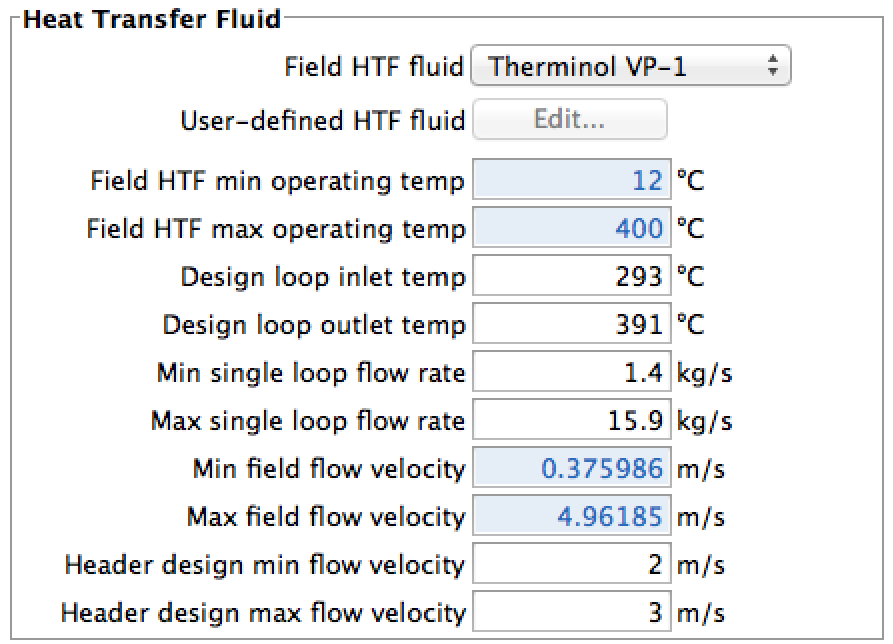
\includegraphics[width=0.6\linewidth]{FIG/PTC_HTF}
\caption[Screenshot of HTF input parameter for SAM.]{Screenshot of HTF input parameter for SAM.}\label{PTC_HTF}
\end{figure}


The size of the solar field is strongly effected by the solar multiple and the thermal demand of the steam Rankine cycle. At a solar multiple of \si{1} (design thermal power of the steam generator) the solar field requires \SI{453003}{\square\metre} ($\approx$\SI{45.3}{ha}) reflective aperture area of SCA. \si{65.86} ($\approx$66) loops are required at a SM of \si{1}. The number of loops and so also the field size multiplies by the value of the SM.



Also the the solar field area and thereby the total land area depending by the SM. Equation~\ref{GL_PTCSolarfieldarea} shows the influence on the solar field area of the ratio between the row spacing and the SCA width. The roe spacing is assumed by \SI{18}{m} between the parallel SCAs. The total land area results by Equation~\ref{GL_PTCtotallandarea} and is the solar field area multiplies by the factor of non-solar field area. The factor is assumed by \si{1.4} in the simulation \cite{NREL2015a}.
\begin{align}
\textrm{solar field area }(m^2) =\textrm{aperture area }(m^2) \times \frac{\textrm{row spacing }(m)}{ \textrm{SCA width }(m)} \label{GL_PTCSolarfieldarea}
\end{align}
\begin{align}
\textrm{total land area }(m^2) =\textrm{solar field area }(m^2) \times  \textrm{non-solar field multiplier}\label{GL_PTCtotallandarea}
\end{align}
Table~\ref{tbl: PTCSolarfield} shows the solar field simulation parameter of the PTC system for the simulation configuration values of the solar multiple. The parameters of the Table comes from the above mentioned relations between the Items. The design power of the steam generator (SG) stays at \SI{318.0}{\mega\wattth} while the solar field thermal output rises proportional through the SM. 
\begin{table}[!h]  
  \centering
	\begin{tabular}{ p{3.3cm} C{1.1cm} C{1.1cm} C{1.1cm} C{1.1cm} C{1.1cm} C{1.1cm} C{1.1cm} C{1.1cm} } 
	\hline	
\textbf{Item} & \textbf{Unit} & \multicolumn{7}{c}{\textbf{Value}} \\ \hline \hline
SG Design power & \si{\mega\wattth} &  \multicolumn{7}{c}{318.0}\\
Design-point DNI & \si{\watt\per\metre} &  \multicolumn{7}{c}{950}\\
\hline
\textbf{Solar multiple} &  & \textbf{2.0} & \textbf{2.5} & \textbf{3.0} & \textbf{3.5} & \textbf{4.0} & \textbf{4.5} & \textbf{5.0}\\ \hline 
Field th. output & \si{\mega\wattth} & 636 & 795 & 954 & 1~113 & 1~272 & 1~431 & 1~590\\
Number of loops  & - & 132 & 165 & 198 & 231 & 264 & 297 & 330\\ 
Aperture refl. area & ha & 90.6 & 113.3 & 135.9 & 158.6 & 181.2 & 203.9 & 226.5\\ 
Total land area & ha & 675 & 845 & 1013 & 1~182 & 1~351 &1~540 & 1~689\\ 
\hline
\end{tabular}
\caption[PTC solar field parameter.]{PTC solar field parameter.}\label{tbl: PTCSolarfield}
\end{table}
\pagebreak
\subsubsection{Thermal energy storage (TES)}
The thermal energy storage (TES) of the simulated PTC system uses a indirect two-tank molten salt system with "Hitec Solar Salt" as storage fluid. This storage fluid is made from sodium nitrate (60~\% NaNO\textsubscript{3}) and potassium nitrate (40~\% KNO\textsubscript{3}). Solar Salt needs an minimum operating temperature of 238\si{\celsius} and and has a maximum operating temperature of 593\si{\celsius}. \cite{Suite2011,Kearney2003}

\begin{table}[htbp]  
  \centering
	\begin{tabular}{ p{3.9cm}  C{1.0cm} C{1.2cm} C{1.2cm} C{1.2cm} C{1.2cm} C{1.2cm} } 
	\hline	
\textbf{Item} & \textbf{Unit} & \multicolumn{5}{c}{\textbf{Value}} \\ \hline \hline
Storage type & - &  \multicolumn{5}{c}{indirect two-tank molten salt}\\
Storage fluid & - &  \multicolumn{5}{c}{Hitec Solar Salt}\\
Hot tank design temp. & \si{\celsius} & \multicolumn{5}{c}{391}\\
Cold tank design temp. & \si{\celsius} & \multicolumn{5}{c}{293}\\
\hline
\textbf{TES full load hours} & \textbf{h} & \textbf{8} & \textbf{10} & \textbf{12} & \textbf{14} & \textbf{16}\\ \hline 
Thermal capacity & \si{\mega\wattth\hour}  & 2~544 & 3~180 & 3~816 & 4~452 & 5~087 \\
Storage volume  & \si{\cubed\metre} & 34~407 & 43~008 & 51~610 & 60~212 & 68~813\\
\hline
\end{tabular}
\caption[PTC system TES parameter.]{PTC system TES parameter.}\label{tbl: PTCTES}
\end{table}

The storage design temperatures depends from the solar field design temperatures, so the designed temperature difference is \SI{98}{K}. As it is shown in Table~\ref{tbl: PTCTES} the operating temperature limits fits with the storage tank design temperatures. The heater set point is 265\si{\celsius} for both storage tanks. The TES full load hours goes from 8 to 16 in steps of 2. The thermal capacity and also the storage volume rises with the TES full load hours. The simulated stored thermal capacity reaches from 2~\SI{544}{MWh}\textsubscript{th}  at 8 full load hours up to 5~\SI{087}{MWh}\textsubscript{th} at 16 full load hours. It is obviously, that the storage volume of the PTC needs to be more than 3 times that much than the storage volume of the CR system. This is the result of lower temperature difference of the HTF and the turbine design capacity.

Also for the simulation of the PTC system the dispatch control of the turbine output fraction in the storage settings was used. Figure~\ref{PTC_turbineoutput} shows the dispatch control matrix for the turbine output fraction.
\begin{figure}[htbp]  
\centering
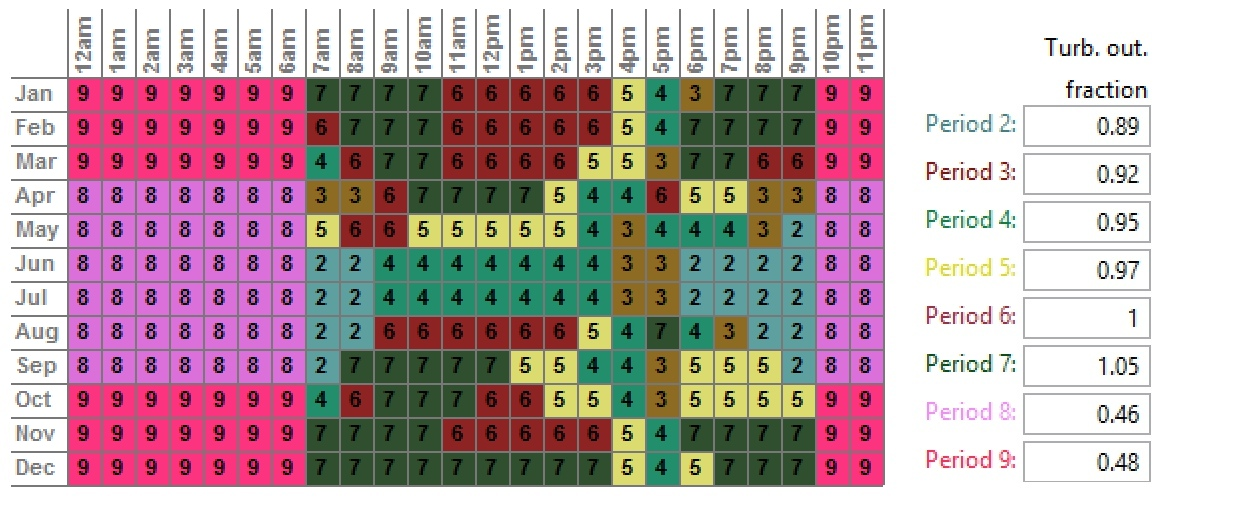
\includegraphics[width=0.95\linewidth]{FIG/PTC_turbineoutput}
\caption[TES dispatch control matrix for turbine output fraction of PTC simulation in SAM.]{TES dispatch control matrix for turbine output fraction of PTC simulation in SAM.}\label{PTC_turbineoutput}
\end{figure}
\subsubsection{Financial parameter}
The financial parameter for calculating the LCOE of the simulated configuration are shown in Table~\ref{tbl: PTCFinance}. As before at the CR is the PTC power plant calculated over a lifetime of \SI{25}{years} using a real interest rate of 7.5~\% \cite{FraunhoferISE2013}. Also the total plant availability of  15~\% once-off surcharge for EPC and contingencies on the total investment costs are equal to the CR \cite{Platzer2014}.



The specific costs for the collector field inclusive HTF-system is assumed with \SI{275}{\usd\per\square\metre} from \cite{Morin2012}. These specific cost could also be reduced by 25~\% by using the assumed cost reduction from Flabeg \cite{FLABEG_FE_GmbH2015}. So the for the simulation assumed costs are highly conservative.


The specific costs for the power block are the same as at the CR but from other sources \cite{Platzer2014}. 

The specific costs of \SI{50}{USD/kWh}\textsubscript{th} for the TES of the PTC are up to 50~\% higher than the CR costs \cite{Platzer2014}. This is reduce to the lower energy density using lower storage temperatures \cite{Steinmann2015}. Other expected specific costs between 35 and \SI{50}{USD/kWh}\textsubscript{th} \cite{Steinmann2012}.

As before Fichtner analyzed also the annual O\&M costs for PTC power plants in SA and results costs of 1.96-1.97~\% of the total investment costs \cite{Fichtner2010}. The value of 2~\% can so also be assumed as conservative.

The costs for the land purchase comes from the "African Agriculture Review" report of the Nedbank Capital, which reported the prices for farmland in SA. For the LCOE calculation of the CSP and PV system was the land purchase costs of 3~\SI{000}{USD/ha} assumed which is based on these report \cite{Cassell2012}.
\begin{table}[!h]  
  \centering
	\begin{tabular}{  p{5.0cm} C{2.0cm} C{1.5cm}  C{1.5cm}  C{4.0cm} } 
	\hline	
\textbf{Item} & \textbf{Symbol}& \textbf{Value} & \textbf{Unit} & \textbf{Source}\\ \hline \hline
Collector field/HTF-system & $c_{CF}$ & 275 & \si{\usd\per\square\metre} & \cite{Morin2012}\\ 
Power block &$c_{PB,PTC}$ & 1000 & \si{\usd\per\kilo\wattel} & \cite{Platzer2014}\\ 
Thermal energy storage & $c_{TES,PTC}$ & 50 & \si{\usd\per\kilo\wattth\hour} & \cite{Platzer2014}\\ 
Land purchase & $c_{LP}$ & 3~000 & \si{\usd\per\hectare} & \cite{Cassell2012} \\ 
Annual O\&M & $f_{O\&M,PTC}$ & 2 & \si{\percent} &\cite{Fichtner2010}\\ 
\hline
Lifetime&$n$ & 25 & \si{\year} & \cite{FraunhoferISE2013} \\ 
Interest rate& $i_{PTC}$& 7.5 & \si{\percent} & \cite{FraunhoferISE2013} \\ 
Annual insurance costs& $f_{ins,PTC}$ & 0.5 & \si{\percent} & \cite{IRENA2012}\\
Surcharge for EPC, project management and risk & $f_{EPC,PTC}$ & 15 & \si{\percent} & \cite{Platzer2014} \\
Total plant availability &$f_{avail,plant,PTC}$ & 96 & \si{\percent} & \cite{Morin2012} \\ 
\hline
\end{tabular}
\caption[Finacial input parameter for PTC-simulation in SAM.]{Finacial input parameter for PTC-simulation in SAM.}\label{tbl: PTCFinance}
\end{table}
\section{Results of PTC power plant simulation} \label{sec.resultsPTC}
This section comprised the results of the simulation from the above designed PTC power plant and there belonging LCOE results. Therefore the load curve covering performance and the belonging load profiles and duration curves are described and analyzed. The goal of these Section is to find the suitable PTC design configuration to reach 90~\% covering of the prescribed load which having the lowest belonging LCOE calculation result.
\subsubsection{Load curve covering}
As it was shown in Table~\ref{tbl: PTC_OverallConfig} on Page~\pageref{tbl: PTC_OverallConfig} the PTC system based power plant was simulated in 35 different configurations, using a SM from 2.0 to 5.0 and 8 to \SI{16}{h} of TES, in order to reach the target of 90~\% load curve covering. This section compares the results of the configuration with the lowest SM and TES hours (SM: 2.0 \& TES: \SI{8}{h}) with the configuration using the highest SM and TES hours  (SM: 5.0 \& TES: \SI{16}{h}) representative for all in between.  

The annual average load curve covering result of the selected simulated PTC configurations is shown in Figure~\ref{PTC_annual_profil}. It can be seen, that the PTC power plant using a SM of 5.0 and \SI{16}{h} of TES covers mostly any time of the year the prescribed load curve. But it is also obviously that power supply declines during the night from \SI{3}{am} on and is also decreasing in the morning hours at \SI{8}{am}. In comparison to that covers the PTC power plant using a SM of 2.0 and \SI{8}{h} of TES significantly less of the year the prescribed load curve. This simulated configuration of the PTC system starts declining the covering directly in the afternoon and standstill during the night from 3 to \SI{6}{am} during the whole year. All annual average load profile simulation results can be found in Appendix~\ref{all_load_profile}.

\begin{figure}[htbp]  
\centering
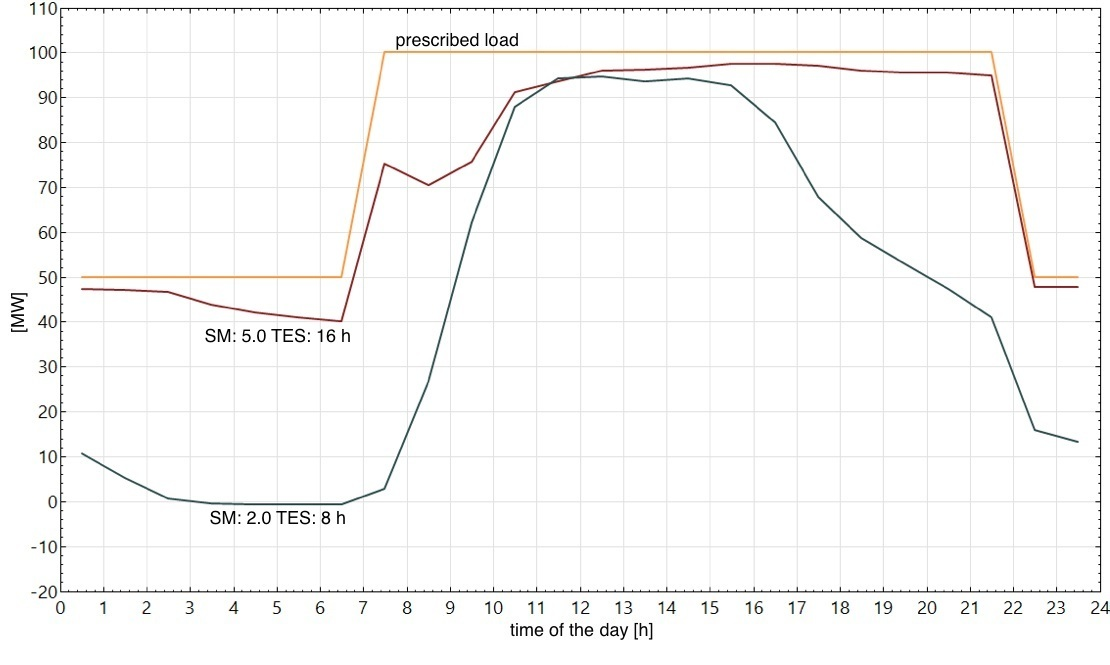
\includegraphics[width=0.8\linewidth]{FIG/PTC_annual_profil}
\caption[Annual average load profile of selected PTC power plant configurations.]{Annual average load profile of selected PTC power plant configurations.}\label{PTC_annual_profil}
\end{figure}
The annual average load curve covering coming from the covering of the prescribed load at any time of the year through the net output of the power plant. The net output variate at any time step and depends on one side from the local whether date and on the other side from the set parameters. The annual sun paths diagram of Upington can be seen on Page~\pageref{SunPathUpington} in Figure~\ref{SunPathUpington}. 

Figure~\ref{PTC_winter_load} shows the load curve behavior of the selected PTC power plant configurations during the time of winter solstice, so the time with the shortest time of sunlight and the lowest angle of the incoming sunlight in Upington, SA. In the portrayed time line the DNI coming fro the whether file has a maximum of a about \SI{830}{\watt\per\square\metre} in peak times and there are also days with lower or almost no direct irradiance. 

The net electricity production of the PTC power plant with low configurations don't reach the prescribed load at any time in this portrayed time line. Therefore it is obviously that the solar field don't collect enough thermal energy during the day for filling up the storage to supply the steam turbines also by night. The power that is produced by the solar field goes at any time directly to the power generation and without direct sun irradiance the production is coming to standstill. The parasitic consumer has a peak load of about \SI{8}{MW} during these days in these configuration.

In comparison to that is reaches the net electricity production of the PTC power plant with high configurations almost everyday the prescribed load for some hours. These configuration can also produce enough thermal energy by the solar field to fill up the storage to produce energy till after midnight. But also in that configuration is coming to standstill every night and rises first with the incoming direct irradiance again. In this configuration there is a peak load of about \SI{12}{MW} coming from the parasitic consumer. 

The overproduction of the net output depends on the gross output control and the variable parasitic consumers. The turbine output was preset for all PTC power plant simulation using the turbine output fraction of the TES dispatch control matrix which illustrated in Figure~\ref{PTC_turbineoutput} on Page~\pageref{PTC_turbineoutput}. So it was not possible to regulate the net output under variable external influences at any time. 

\begin{figure}[htbp]  
\centering
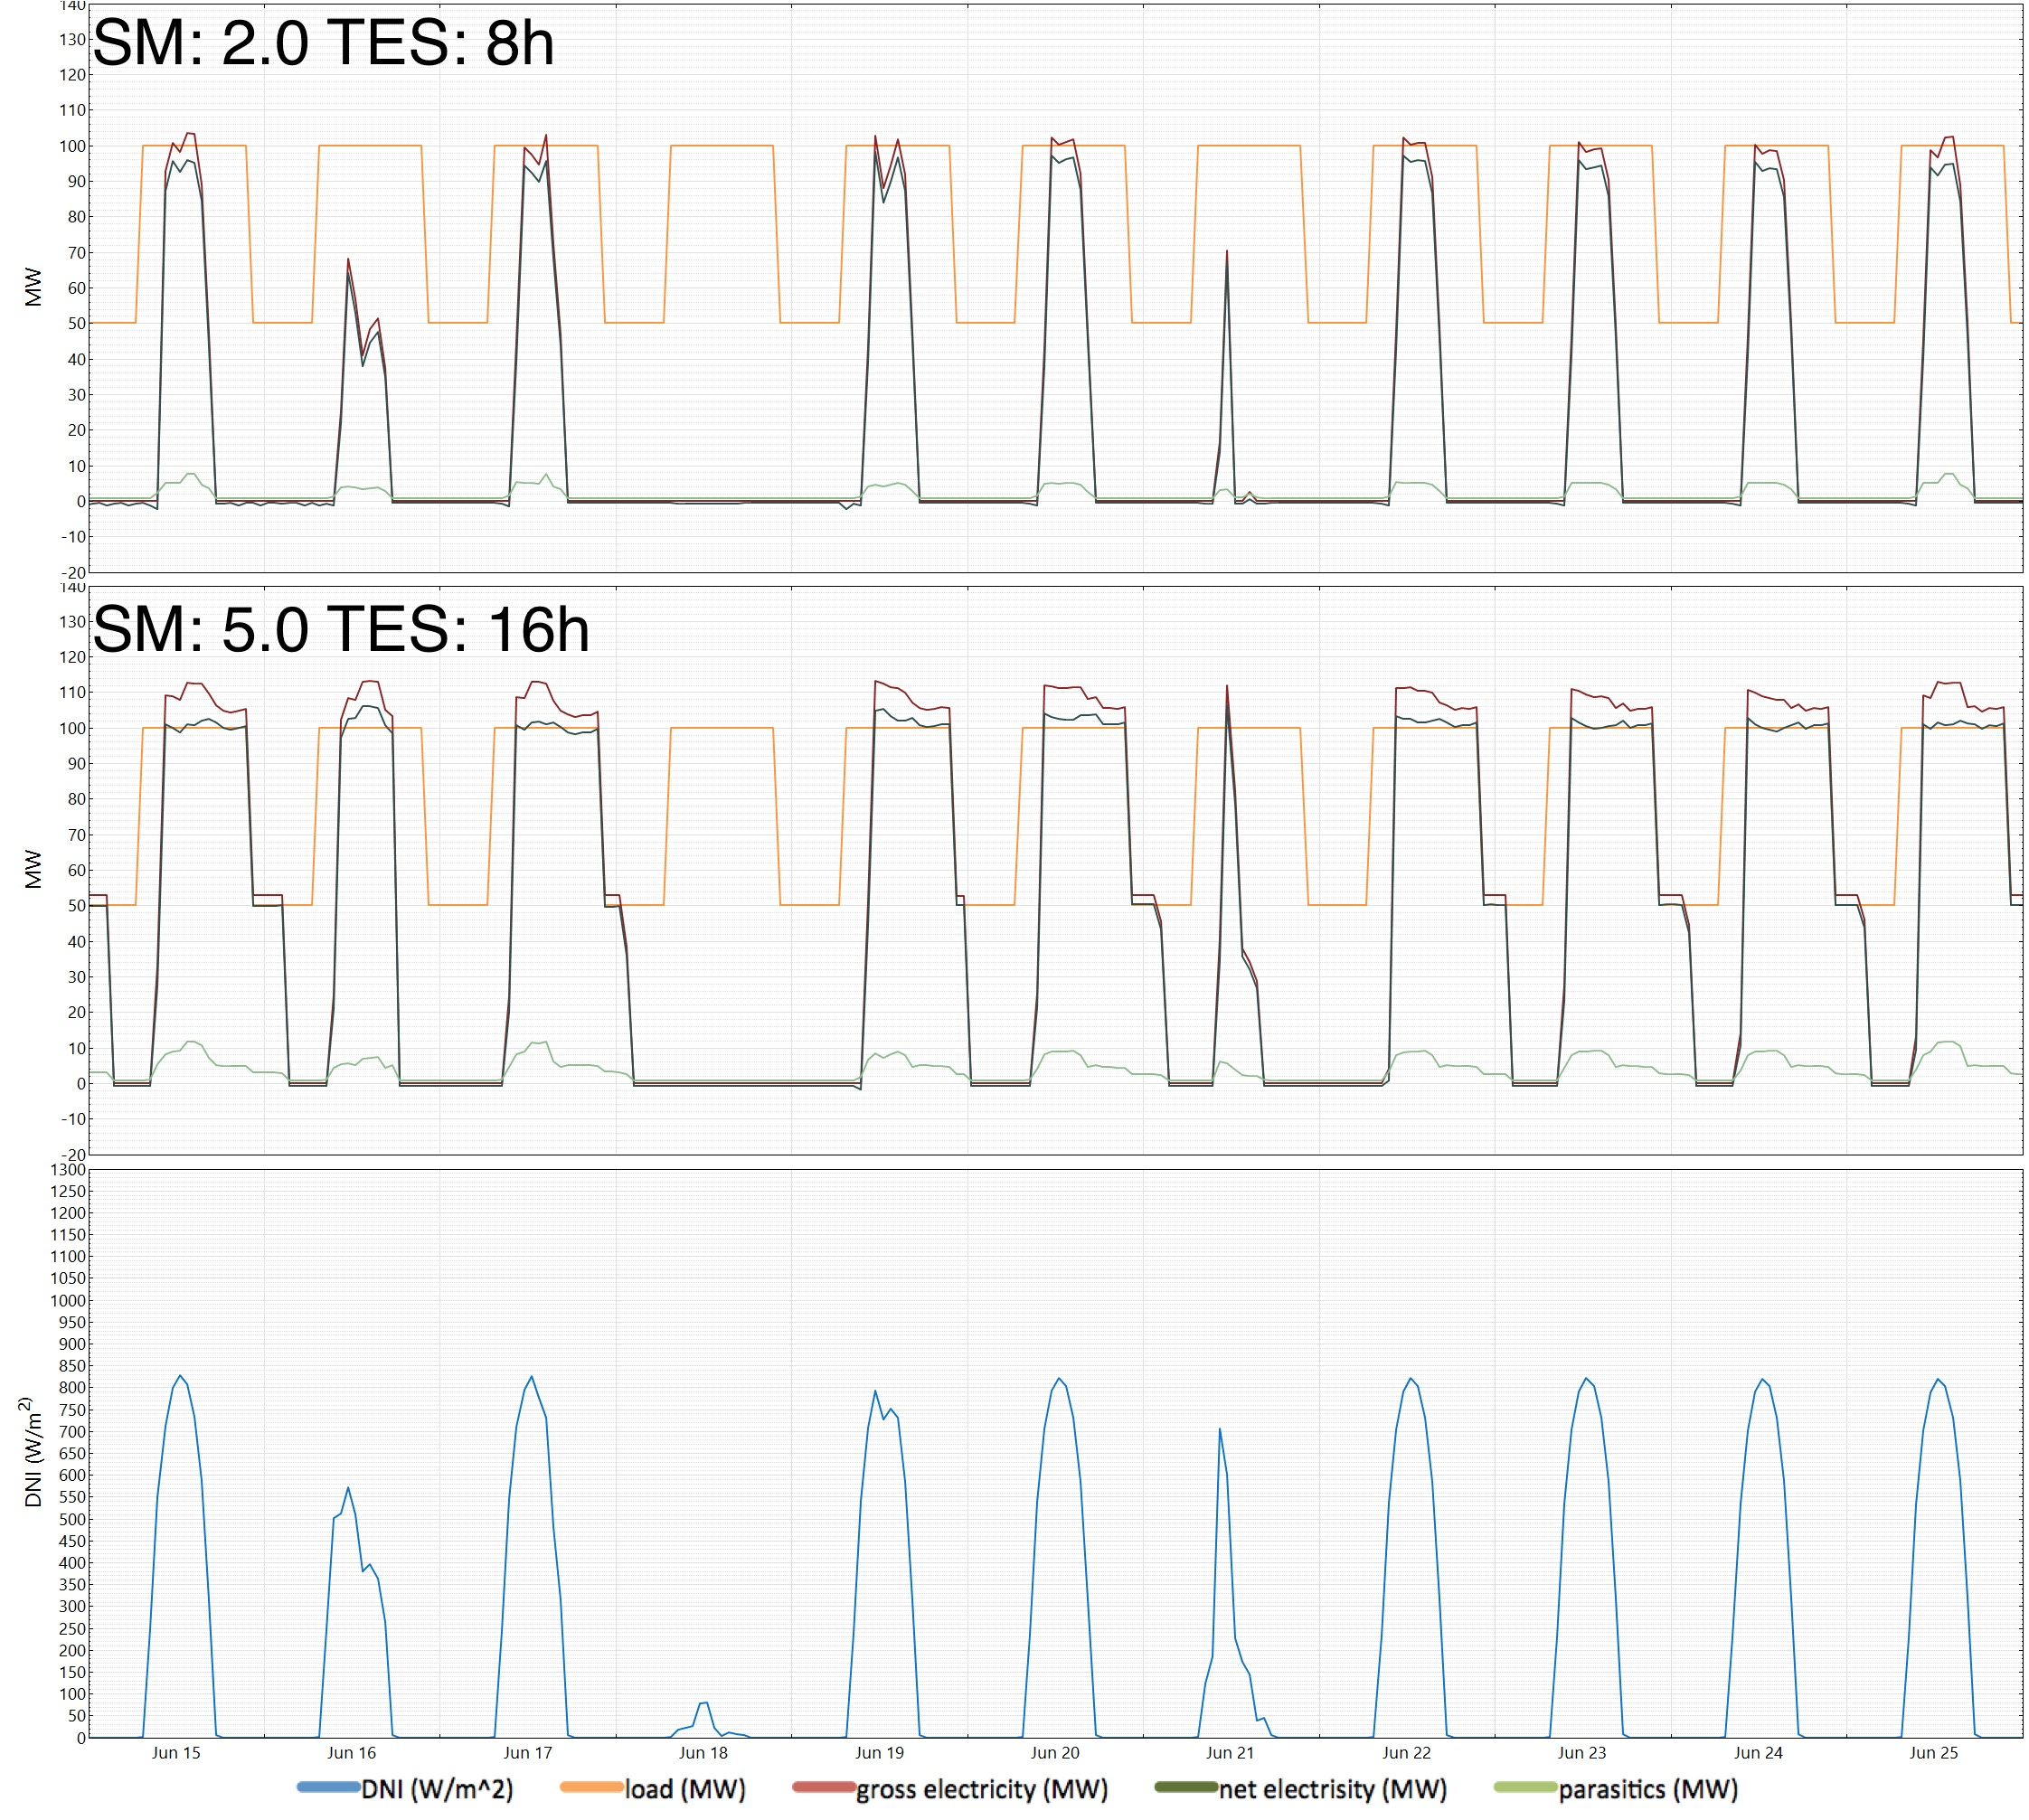
\includegraphics[width=1\linewidth]{FIG/PTC_winter_load}
\caption[PTC load profile during the time of winter solstice (15. June - 25. June).]{PTC load profile during the time of winter solstice (15. June - 25. June).}\label{PTC_winter_load}
\end{figure}
It is obviously that the performance of the PCT power plant isn't great at all during the winter solstice. Neither under high then low performance configurations. This leads mainly from the declining optical performance of the solar collector field under impact of lower sunlight angle during the winter months. This performance loss can mainly reduce to the cosine efficiency of the solar field. Figure~\ref{PTC_field_eff} gives an impression of the strong influence of the cosine efficiency on the total optical field efficiency of the simulated PTC power plants. It can be seen that the cosine effect reduces the total field efficiency by almost 50~\% during the midday in June. 

\begin{figure}[!htbp]
        \centering                
        \begin{subfigure}[b]{0.5\textwidth}
                \centering
                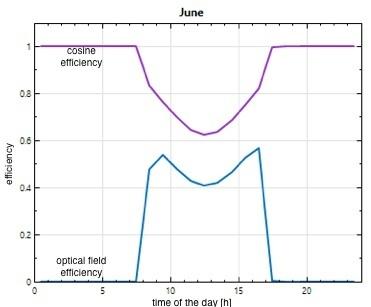
\includegraphics[width=1\textwidth]{FIG/PTC_field_eff_winter}
                \caption{Avarage influence of the cosine efficiency on the avarage total optical field efficiency in June.}\label{PTC_field_eff_winter}
        \end{subfigure}%
        ~
        \begin{subfigure}[b]{0.5\textwidth}
                \centering
                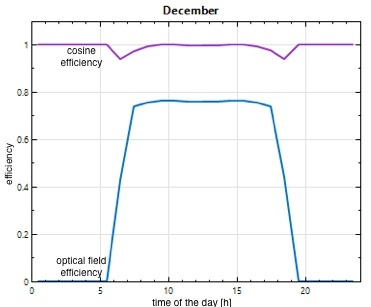
\includegraphics[width=1\textwidth]{FIG/PTC_field_eff_summer}
                \caption{Avarage influence of the cosine efficiency on the avarage total optical field efficiency in December.}\label{PTC_field_eff_summer}
        \end{subfigure}
        \caption[Avarage influence of the cosine efficiency on the avarage total optical field efficiency of a PTC power plant for different months of the year.]{Avarage influence of the cosine efficiency on the avarage total optical field efficiency of a PTC power plant for different months of the year.}\label{PTC_field_eff}
\end{figure}
The loss in optical field performance by the cosine effect arise from the low angle of sunlight, therefor is the efficiency loss in the summer months through the cosine effect comparability low and has just an low effect in the morning and evening hours. 

The load behavior of the two exemplary PTC power plants during the summer solstice is shown in Figure~\ref{PTC_summer_load}. It is obviously that the higher values of the DNI which reaches 1~\SI{150}{\watt\per\square\metre} in peak and the better field efficiency leads to a considerably higher covering of the prescribed load in both configurations. 

The lower PTC configuration which is using a SM of 2.0 and \SI{8}{h} of TES can cover almost the full daytime load and a part of the night time load eith the net electricity production. But under this configuration the PTC power plant can't cover the prescribed load during the night at the best irradiance time of the year, therefrom is also the mentioned gap in production in the annual average load curve coming which was mentioned at the beginning of these section. The net electricity production over-scaled prescribed load at the beginning of the days which leads from the mentioned gross power output control. The parasitic consumers reaching a peak demand of \SI{15}{MW} in this configuration. 

Figure~\ref{PTC_summer_load} shows also the load behavior of the PTC power plant with the highest simulated configuration, which doesn't stand still in this portrayed time span. The graph shows that the net out put is not constant at all. This is coming from the gross power output control and from the massive rises from the parasitic consumers, especially the solar field HTF pump. These pump needs to move a high volume of HTF through the HCEs. At a SM of 5.0 the solar field produce 5 times that much heat then the steam turbine actually needs at the design point. This over-scaling is necessary for the energy production in winter times during the night. Therefore the fractions of focused SCA's getting reduced when the generated energy filled up the storage completely and no more energy in demanded by the steam turbine. This is what  happens to the total parasitic consumption in the chart. The fractions of focused SCA's getting reduced so the power of solar field HTF pump is getting reduced as well. The peak of the parasitic consumers reaching a demand of about \SI{33}{MW} which makes about 27.5~\% of the gross turbine capacity.

\begin{figure}[htbp]  
\centering
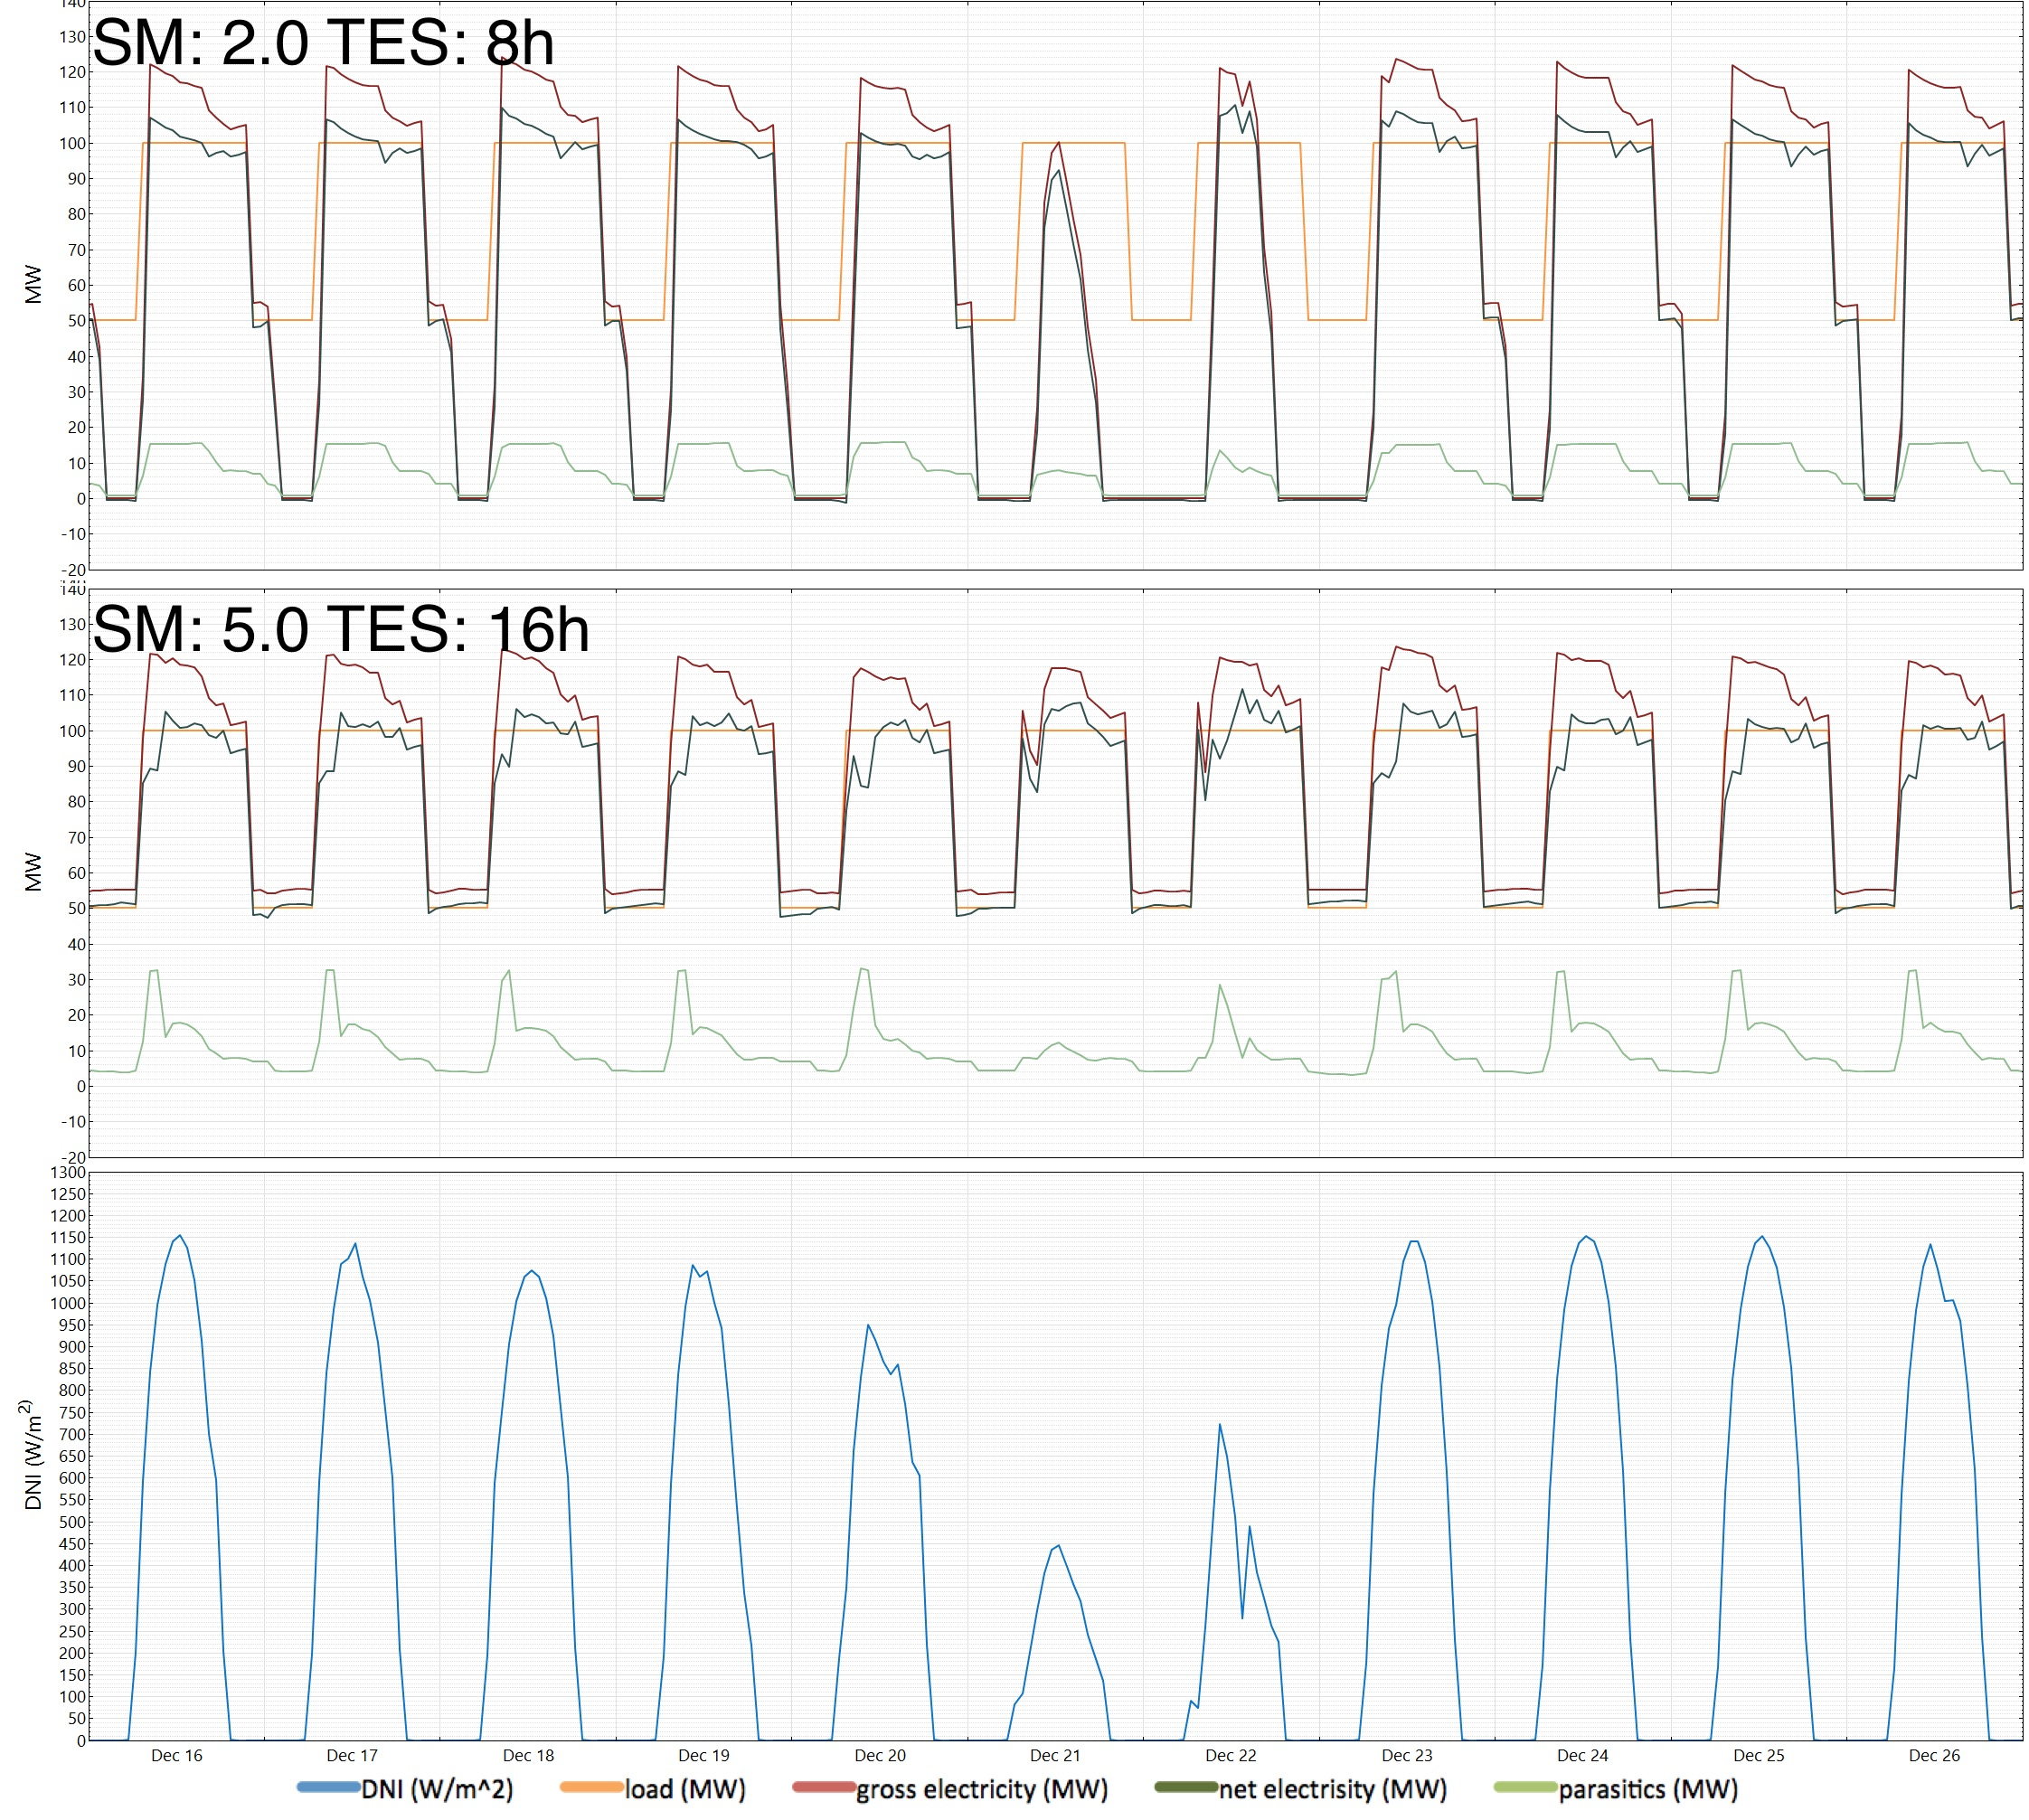
\includegraphics[width=1\linewidth]{FIG/PTC_summer_load}
\caption[PTC load profile during the time of summer solstice (16. December - 26. December).]{PTC load profile during the time of summer solstice (16. December - 26. December).}\label{PTC_summer_load}
\end{figure}
The parasitic demand is composed from different electrical loads of the PTC power plant. Dominantly is the mentioned solar field HTF pump but also the condenser operation of the power cycle. Additionally are the parasitic consumption of the TES \& cycle HTF pump, the field collector drives and the fixed loads. Figure~\ref{PTC_parasitics} shows the share of the produced gross energy of the selected configurations for the simulated year. About 10~\% of the annual gross energy production is going to the parasitic consumers. Therefrom goes about one-third respectively to the condenser operation and the solar field HTF pump. The reaming parasitic load is shared by the TES \& cycle HTF pump and the fixed loads. The share of the field collector drives to the parasitic loads is below 1~\% in any case.

\begin{figure}[!thbp]
        \centering   
        \begin{subfigure}[b]{0.65\textwidth}
                \centering
                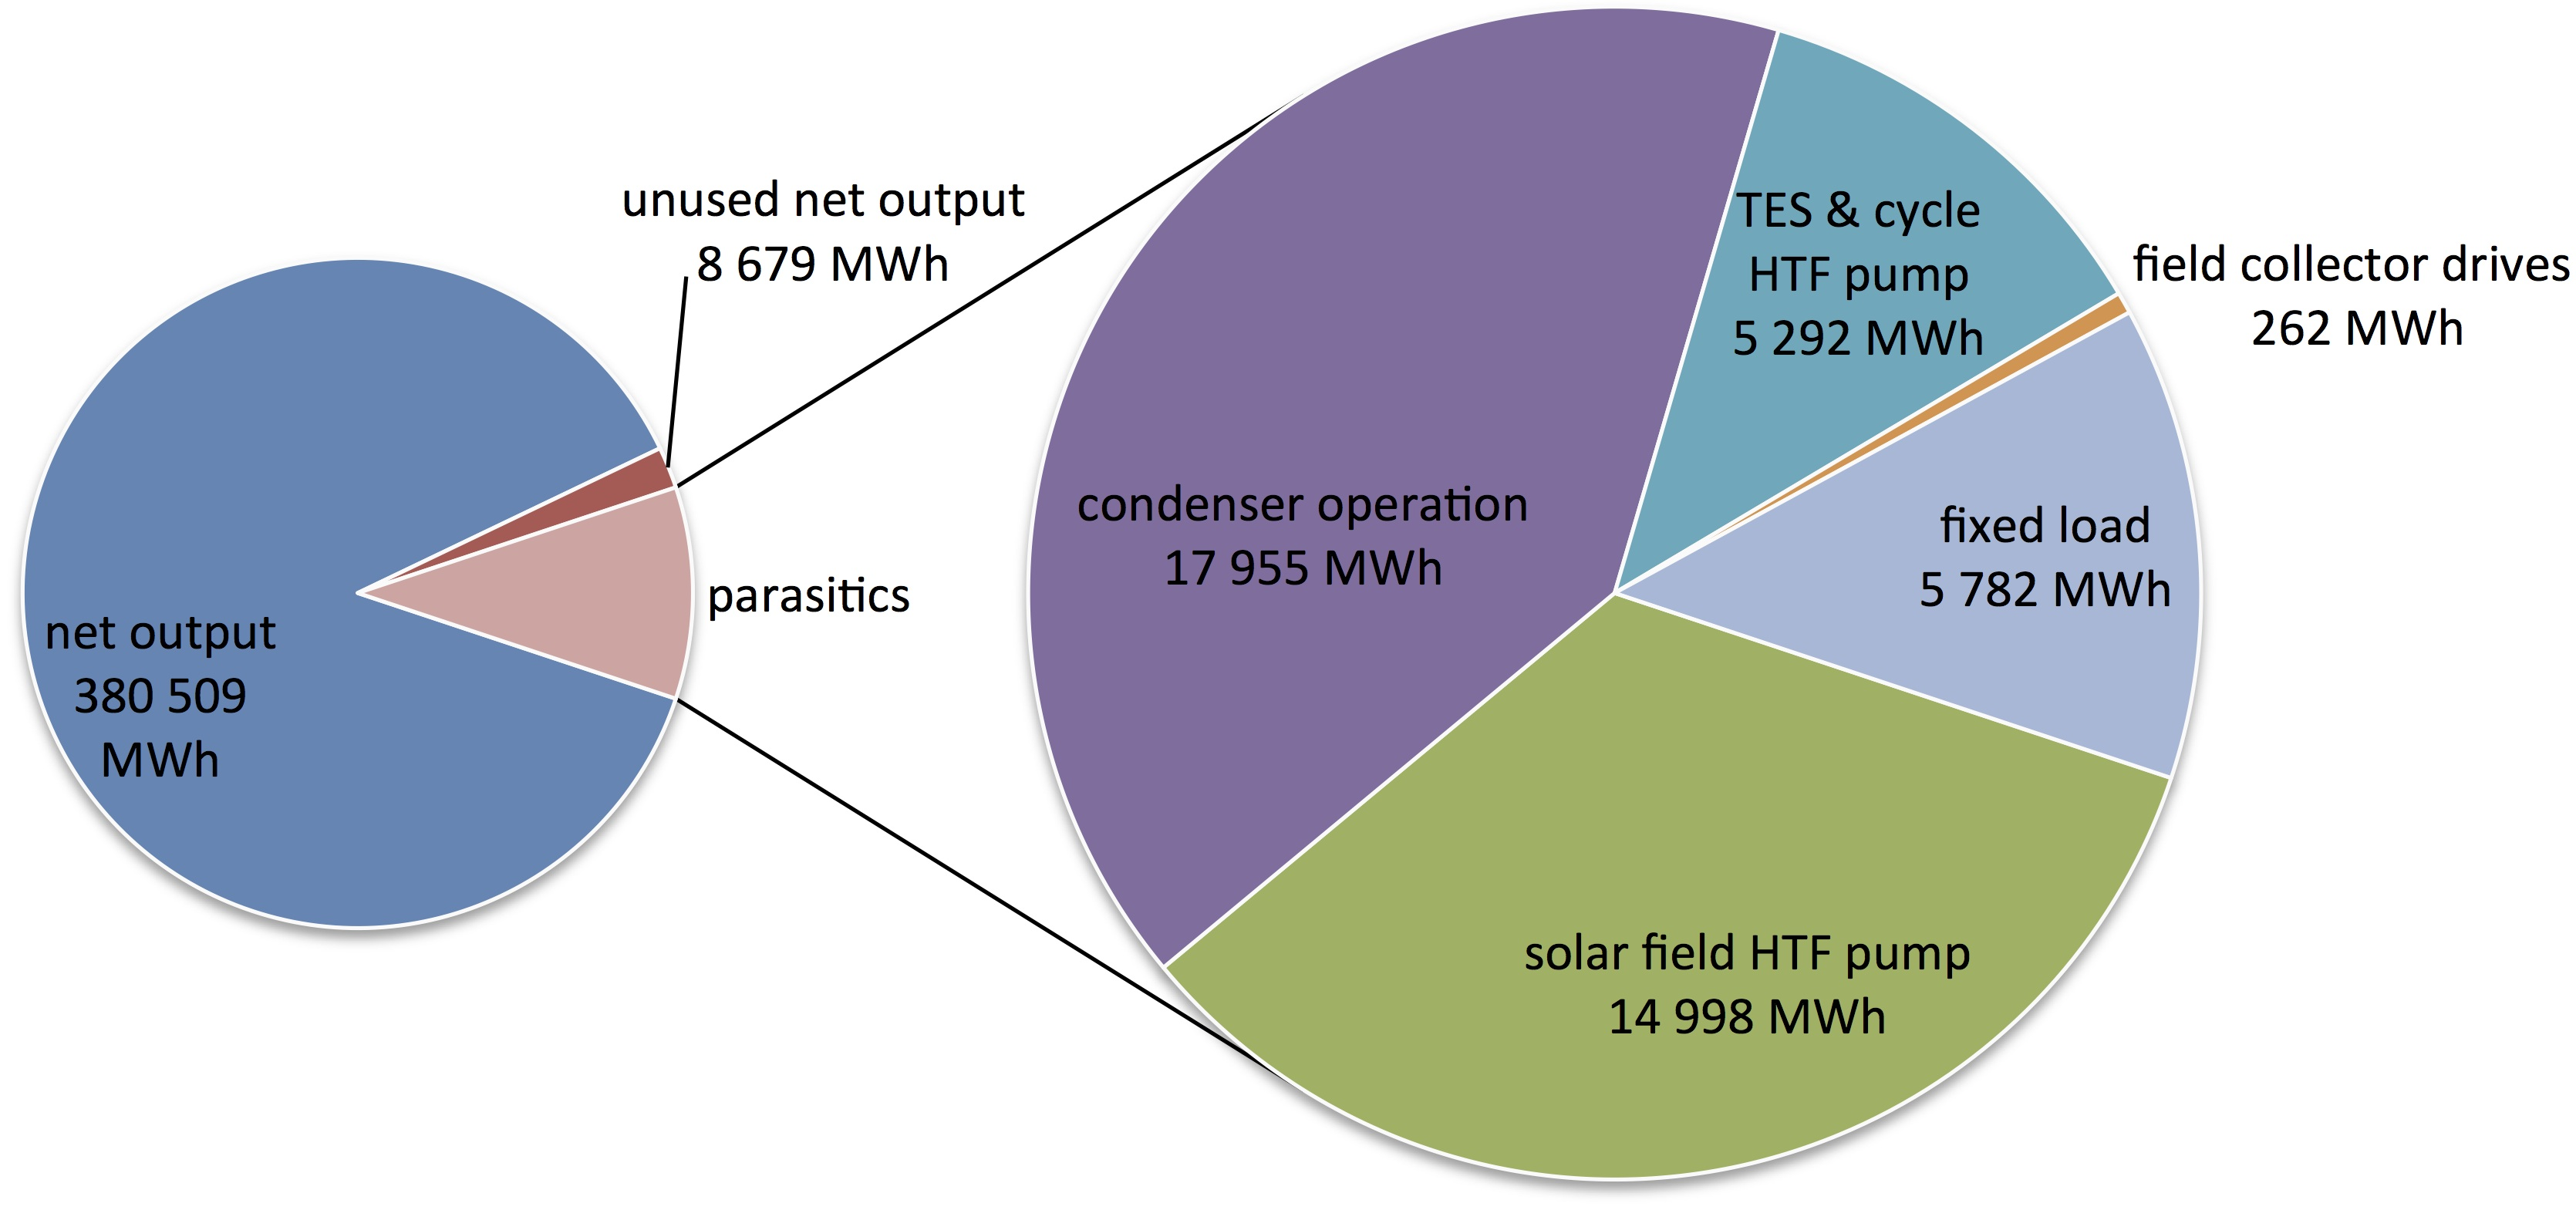
\includegraphics[width=1\textwidth]{FIG/PTC_parasitics_low}
                \caption{SM: 2.0 TES: 8 h}\label{PTC_parasitics_low}
        \end{subfigure}
\par\medskip % Linebreak              
        \begin{subfigure}[b]{0.65\textwidth}
                \centering
                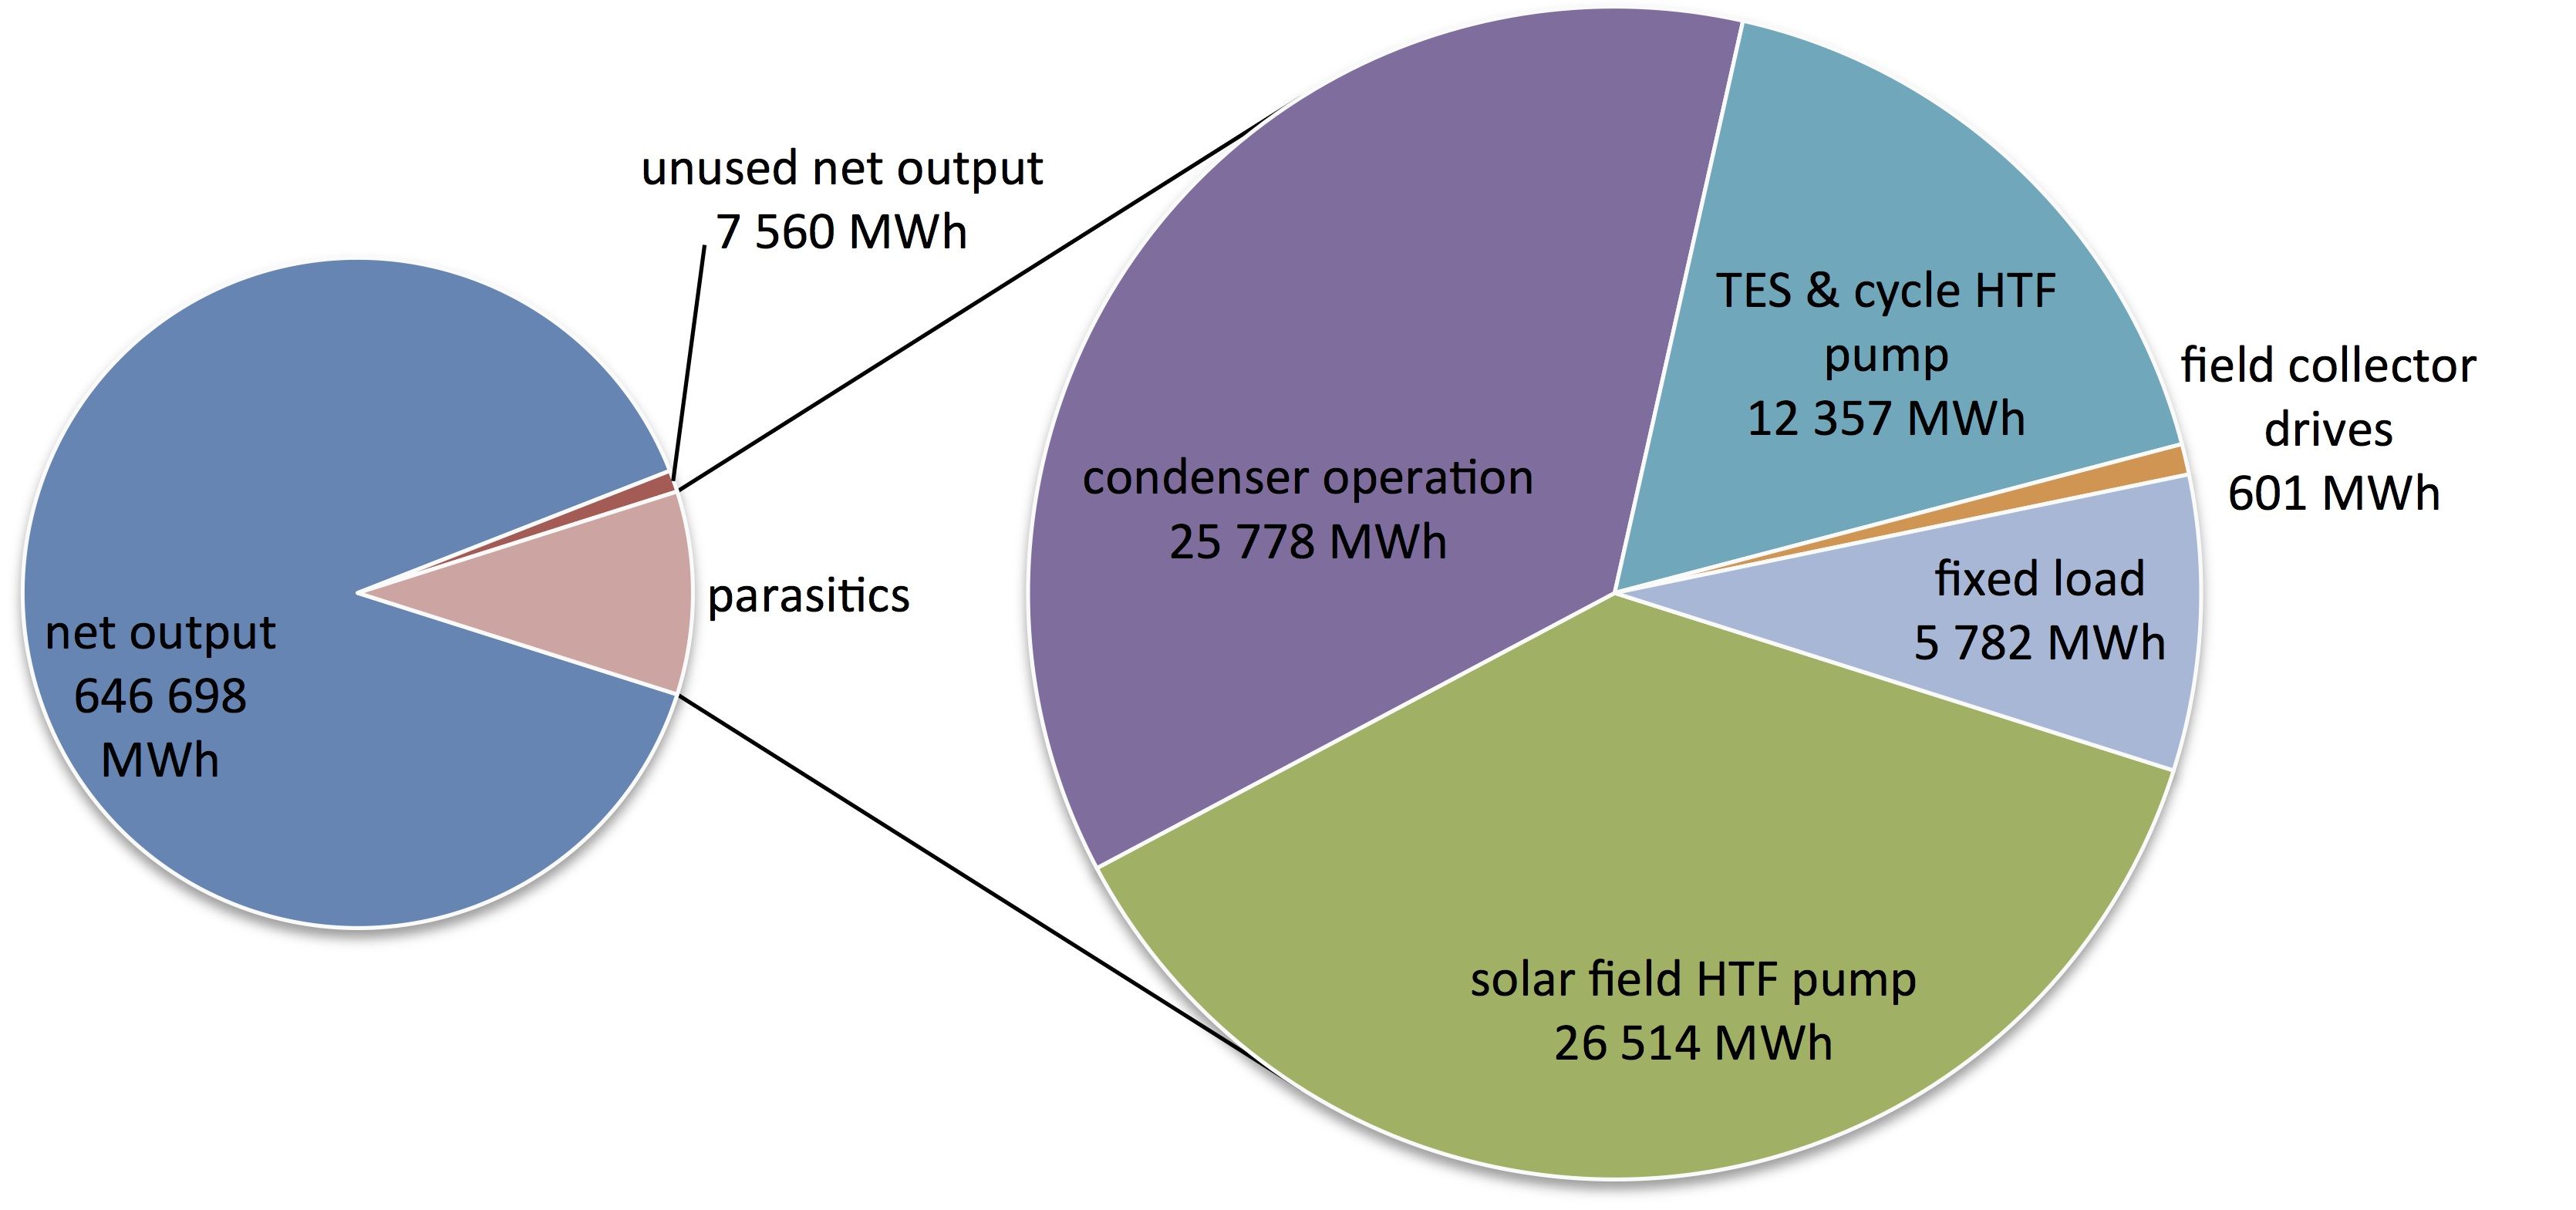
\includegraphics[width=1\textwidth]{FIG/PTC_parasitics_high}
                \caption{SM: 5.0 TES: 16 h}\label{PTC_parasitics_high}
        \end{subfigure}
        \caption[Share of annual gross energy output of selected PTC power plant configurations.]{Share of annual gross energy output of selected PTC power plant configurations.}\label{PTC_parasitics}
\end{figure}
Figure~\ref{PTC_parasitics_low} names the total net output for covering the prescribed load at about \SI{380.51}{GWh} for the PTC power plant with a SM of 2.0 and \SI{8}{h} of TES. The total sum of the annual prescribed load is \SI{711.75}{GWh}. Therefrom results a covering of 53.5~\% of the PTC power plant with the lowest configurations. The annual net output result of the highest simulated PTC configuration can be found in Figure~\ref{PTC_parasitics_high} and is about \SI{646.70}{GWh} which results in a load covering from about 90.9~\% over the year of the prescribed load. 

The remaining load covering results of all simulated PTC power plants can be found in Figure~\ref{PTC_LCCF}. The chart shows that at a SM of 2 all simulated TES variations reaching a load curve covering of 53.4~\%. It can be noteced that the growing rate of the covering is declining with the rising SM. The growing rate from the SM 2.0 to 2.5 is between 10.9~\% and 14.9~\% while it is from the SM 4.5 to 5.0 just between 1~\% and 2~\%. Also there is no noticeable gain between using 12, 14 or \SI{16}{h} of TES. The difference is at highest 0.7~\%. 

\begin{figure}[htbp]  
\centering
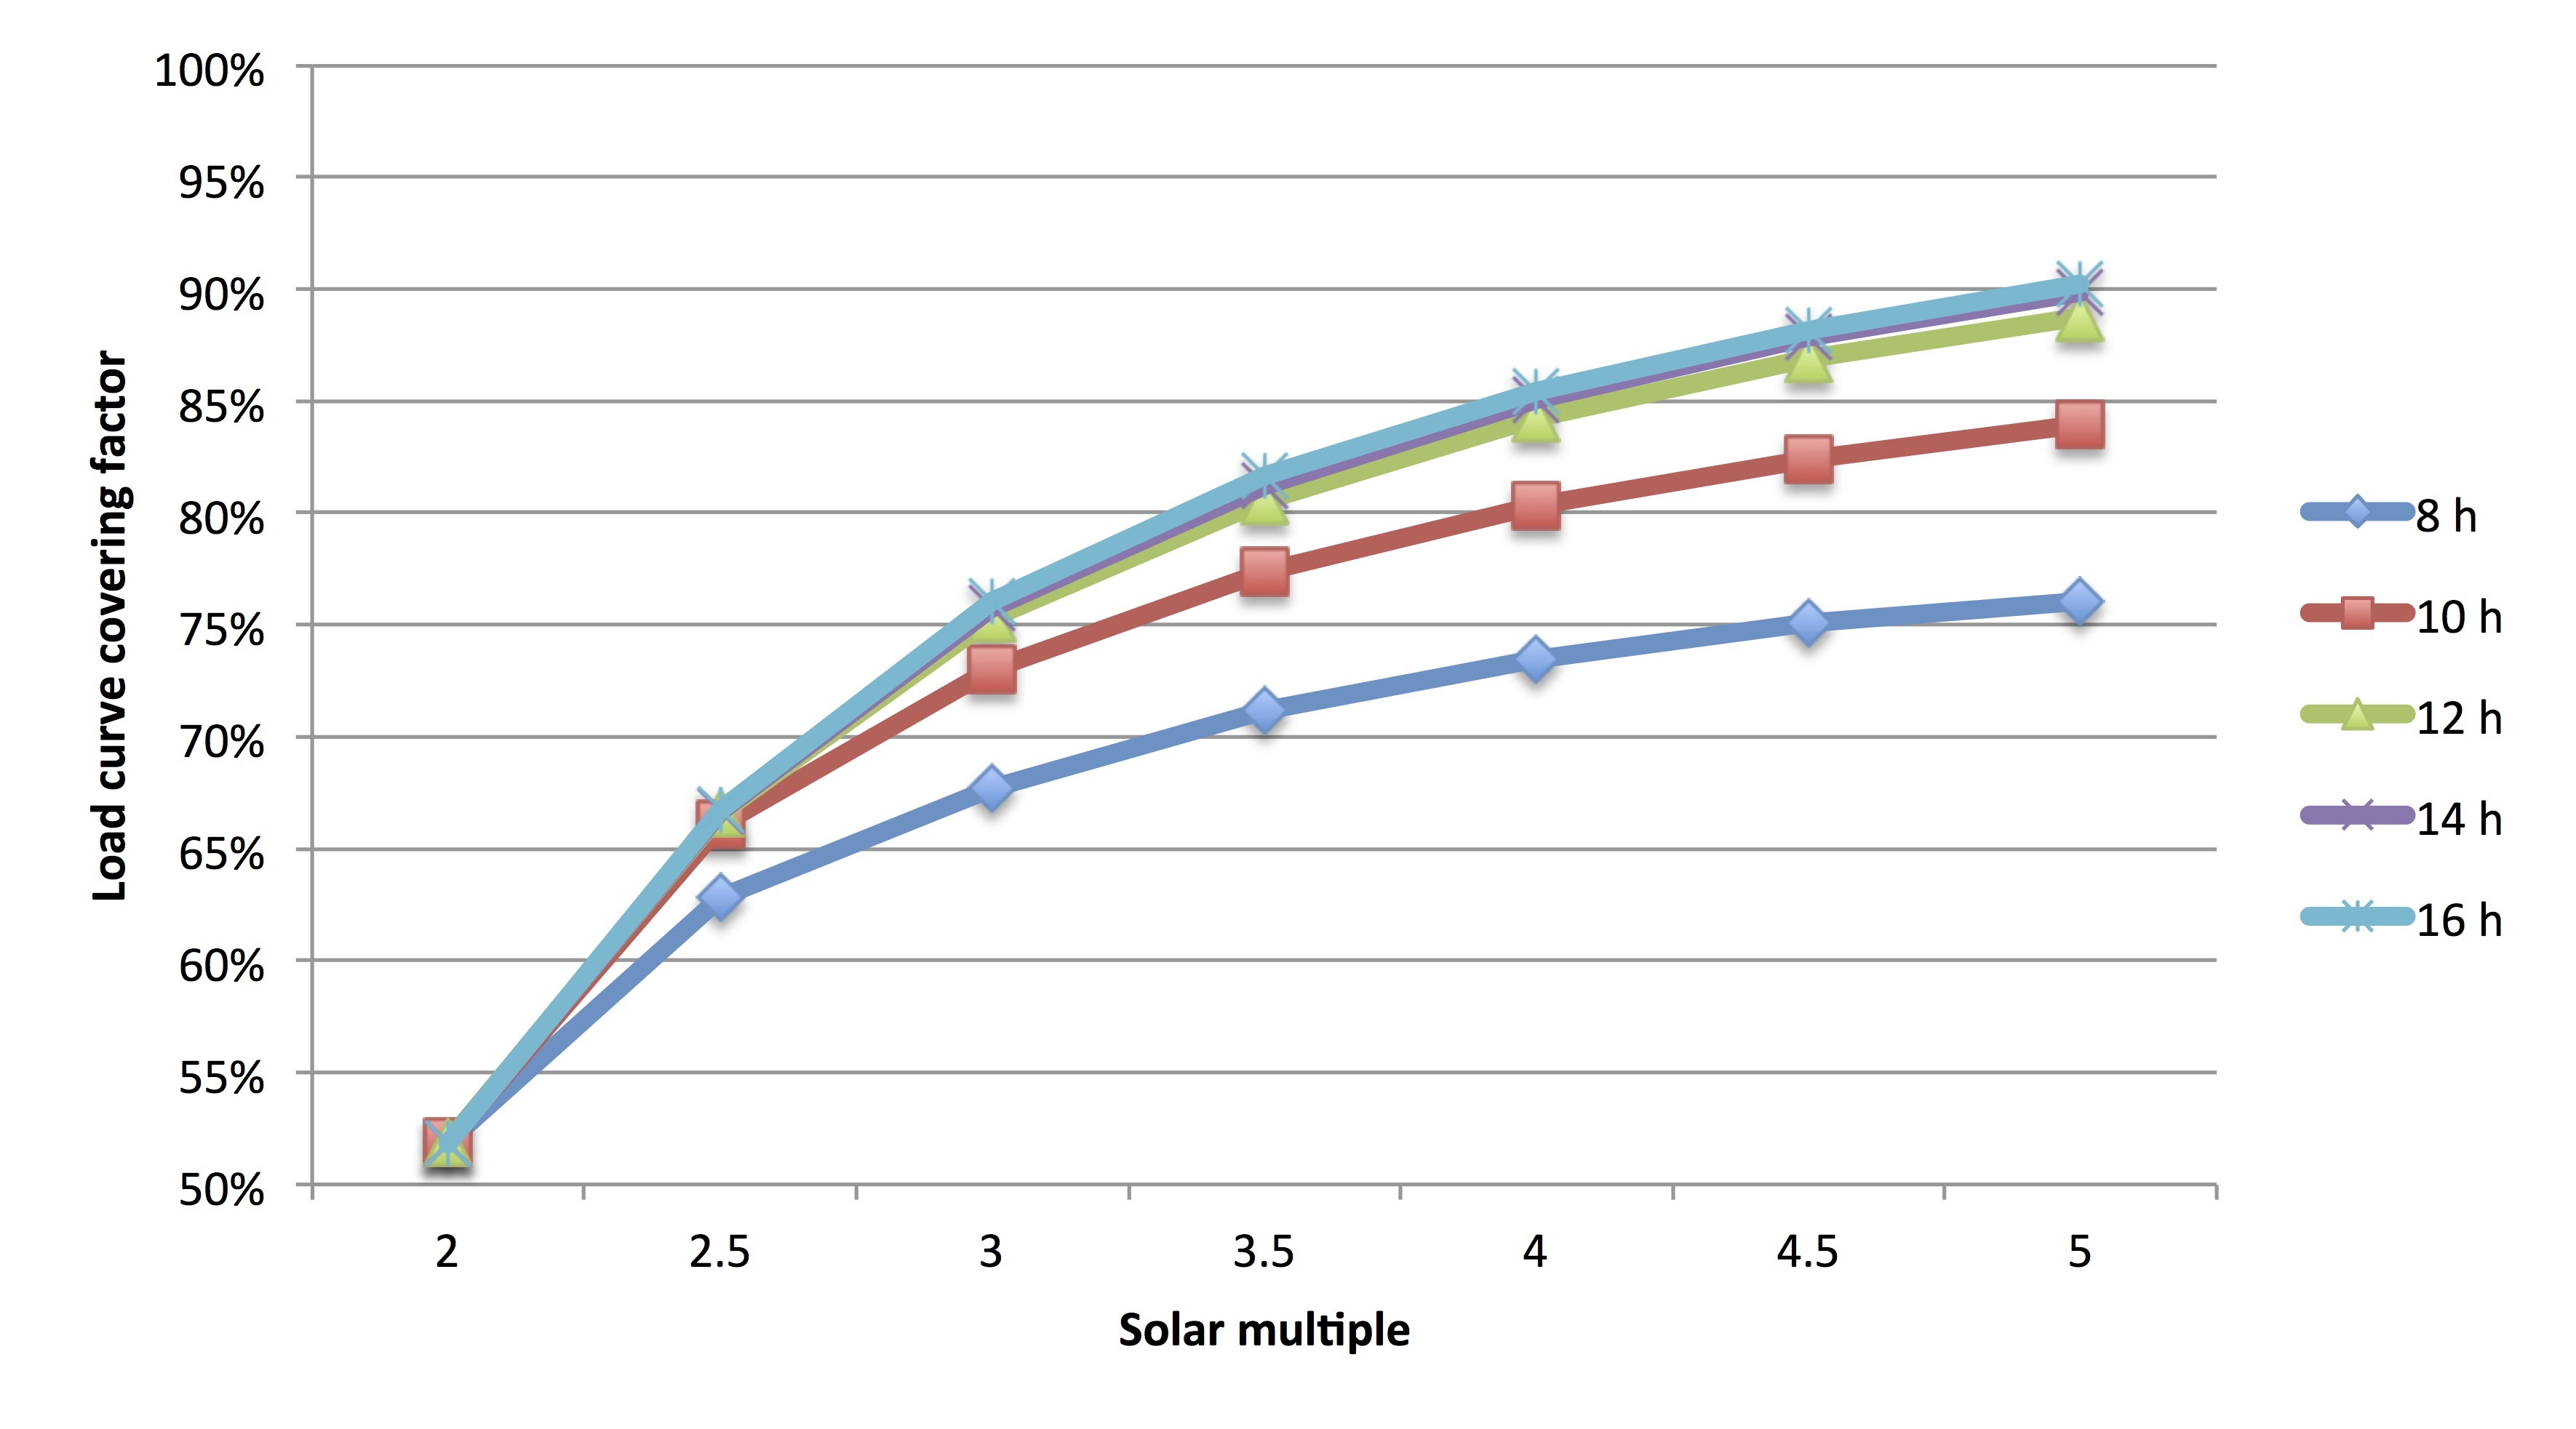
\includegraphics[width=1\linewidth]{FIG/PTC_LCCF}
\caption[Load curve covering result of simulated PTC systems.]{Load curve covering result of simulated PTC systems.}\label{PTC_LCCF}
\end{figure}
The target of 90~\% load covering is just reached by a SM of 5.0 and more then \SI{12}{h} of TES and it can be noted that it seams to be really elaborate for reaching that high value of annual covering using a PTC plant. 70~\% load covering was reached at all simulated PTC configurations. While 80~\% load covering was reached by all configurations besides the \SI{8}{h} of TES.
\subsubsection{Levelized costs of electricity}
For the calculated LCOE the finacial input parameter in Table~\ref{tbl: PTCFinance} and a simplified method which is documented in Appendix~\ref{ChapterLCOE} on Page \pageref{ChapterLCOE} was used. These results of the LCOE claculation for the simulated PTC configurations can be seen in Figure~\ref{PTC_LCOE}. 

The lowest LCOE result of the simulated PTC power plants is \SI{161.69}{USD/MWh} at a SM of 2.5 and \SI{8}{h} of TES. The \SI{10}{h} TES has marginal higher result using a SM of 3.0 (\SI{162.00}{USD/MWh}) and 2.5 (\SI{162.35}{USD/MWh}). The highest LCOE result of \SI{216.63}{USD/MWh} was reached at a SM of 2.0 and \SI{16}{h} of TES. 

Depending from almost identical load curve covering is the behavior of LCOE results of the simulated TES variations 12, 14 and \SI{16}{h} almost identical. The difference in the height of the charts results from the higher investment cost of the larger storage configuration.

\begin{figure}[htbp]  
\centering
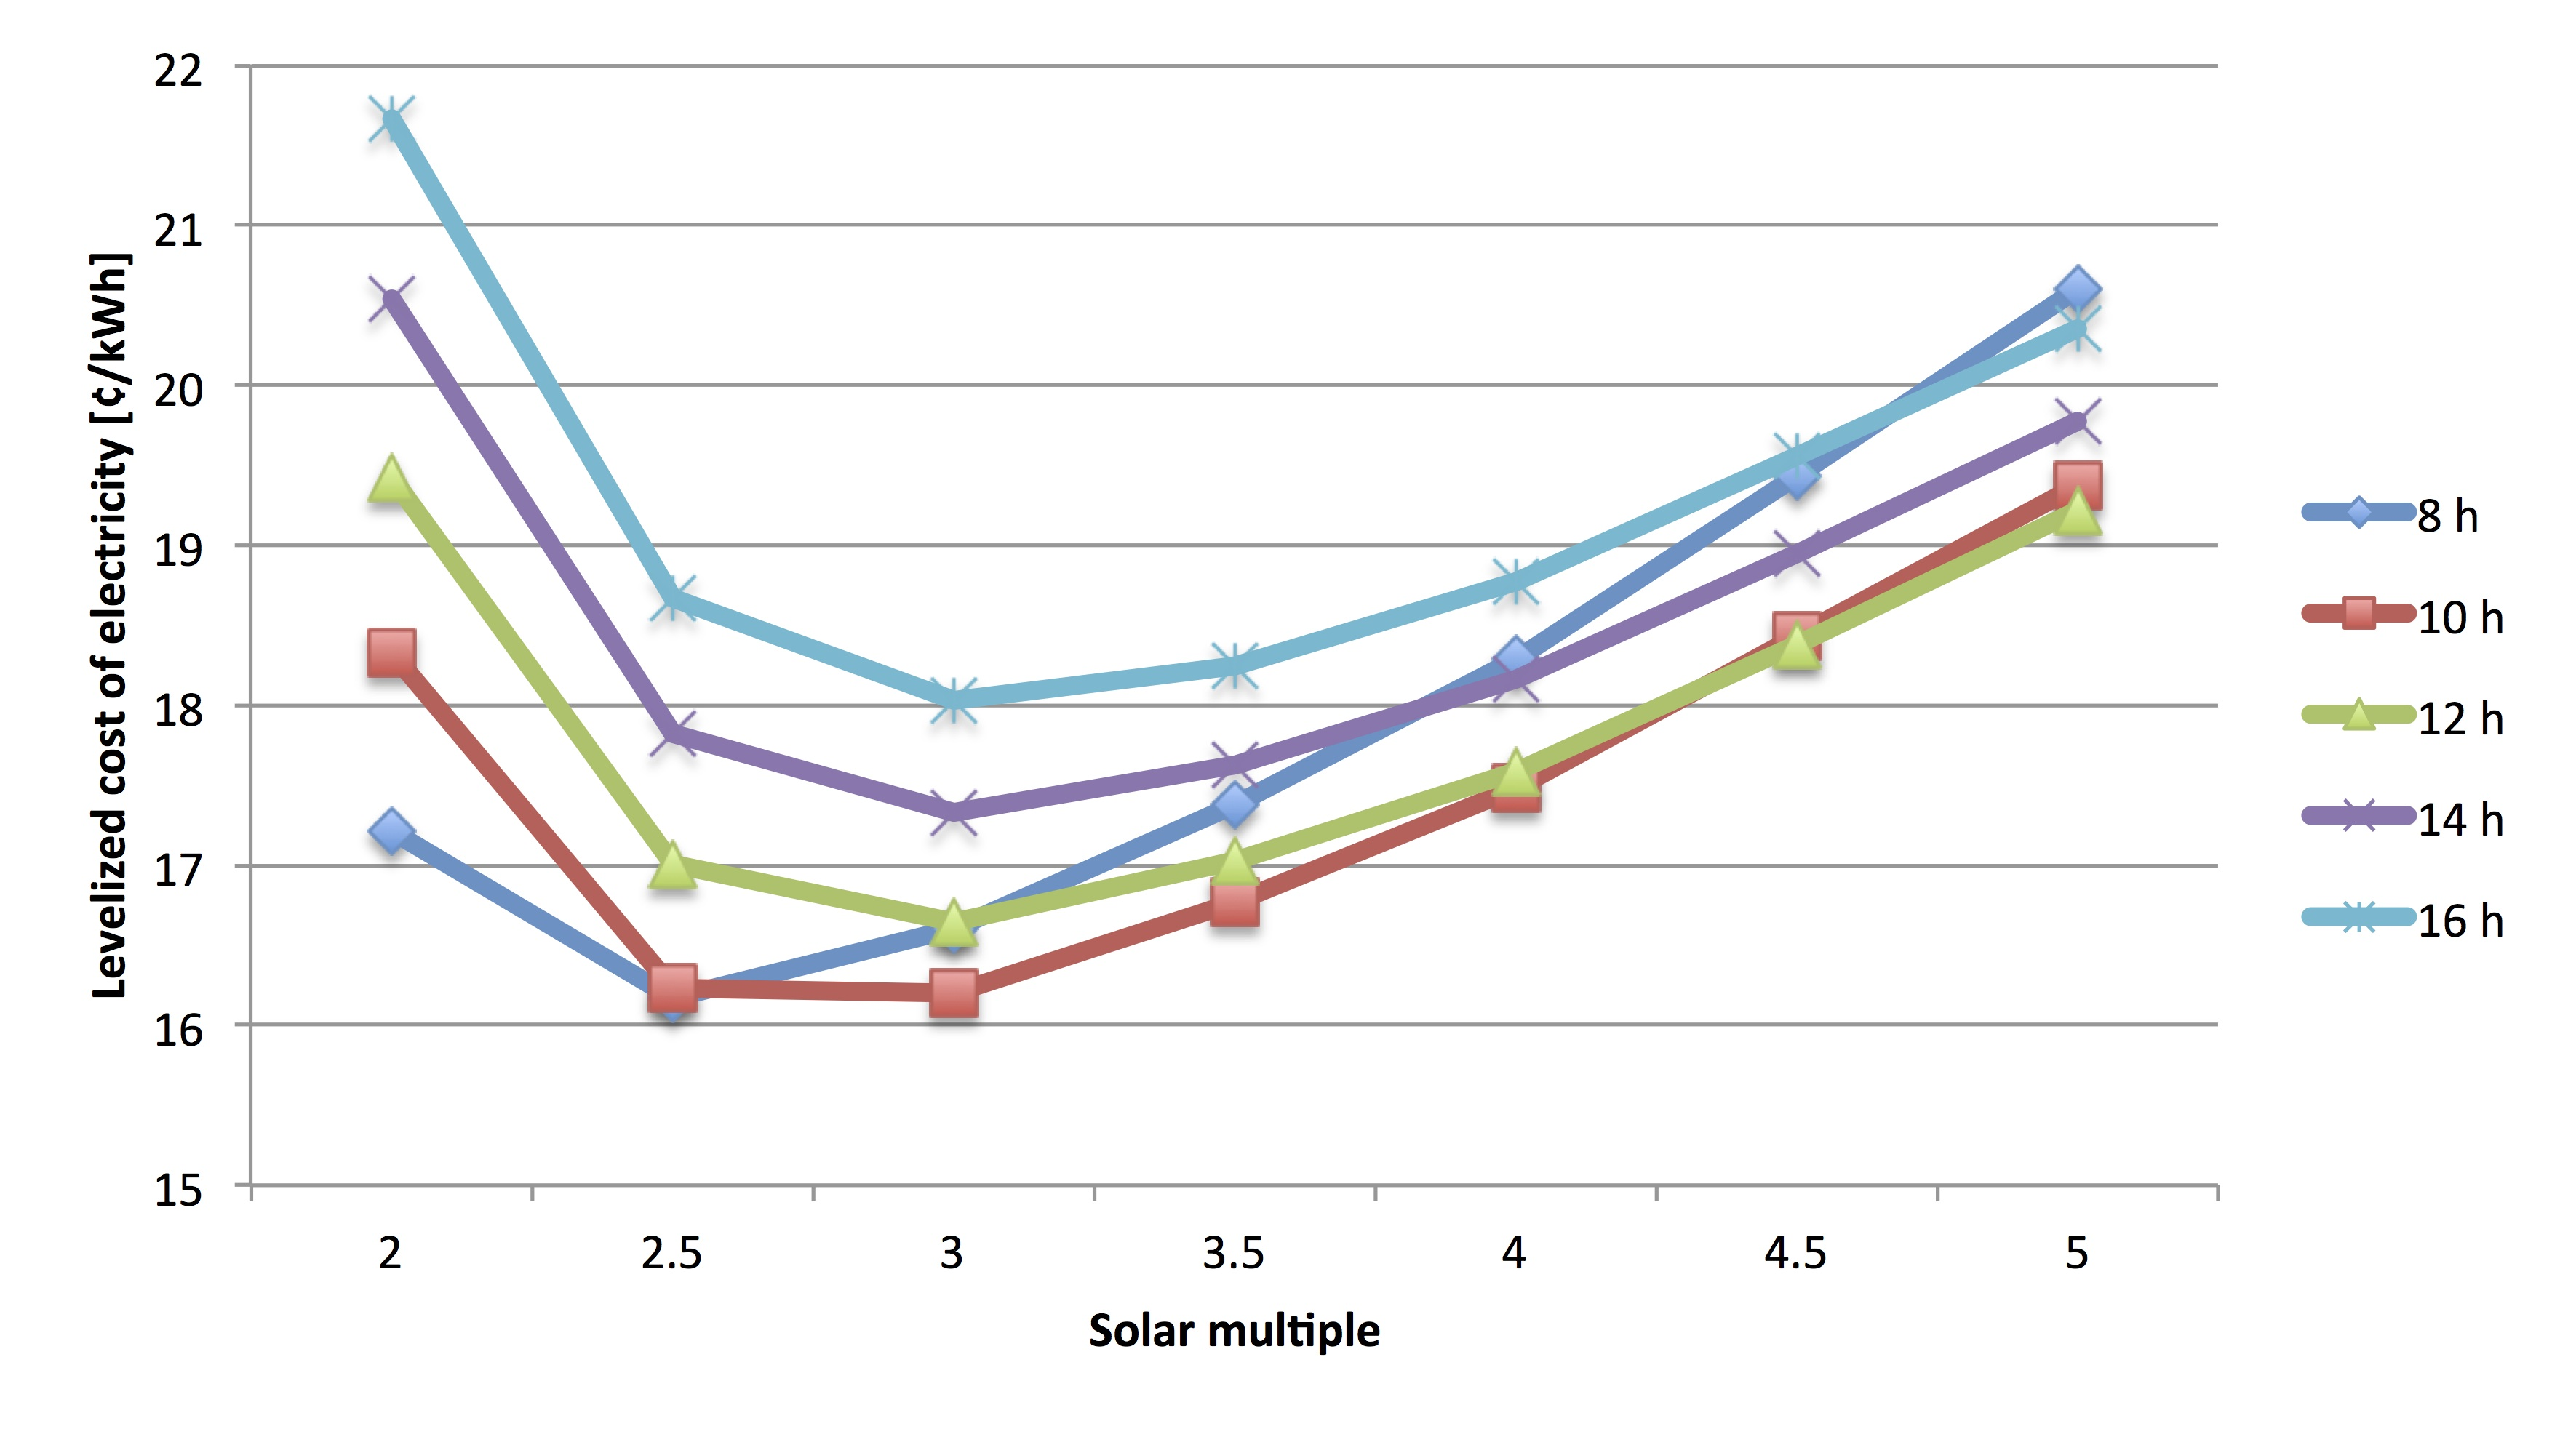
\includegraphics[width=1\linewidth]{FIG/PTC_LCOE}
\caption[LCOE calculation results for PTC simulation.]{LCOE calculation results for PTC simulation.}\label{PTC_LCOE}
\end{figure}
The calculated annual LCOE's of the simulated PTC power plants are composed by six cost parts, namely the investment costs of the collector field, TES, power block, land purchase and additional EPC, project management (PM) and risk as well as the annual operation and maintenance (O\&M) costs. The share of the annual LCOE for the selected PTC power plants can be seen in Figure~\ref{PTC_LCOE_BreakDown}. The share of the land purchase is almost irrelevant for the LCOE. 

When comprising the load curve covering results and the LCOE calculation results of the simulated PTC power plants, the lowest LCOE for reaching the target of 90~\% load curve covering is \SI{192.15}{USD/MWh} at a SM of 5.0 and \SI{16}{h} of TES. 

For reaching a covering of 80~\% of the load curve the PTC configuration with a SM of 3.5 and \SI{12}{h} of TES has the lowest LCOE with \SI{170.32}{USD/MWh}. The lowest LCOE for reaching 70~\% of the prescribed load curve is \SI{162.00}{USD/MWh} at a SM of 3.0 and \SI{10}{h} of TES.
\begin{figure}[!htbp]
        \centering                
        \begin{subfigure}[b]{0.5\textwidth}
                \centering
                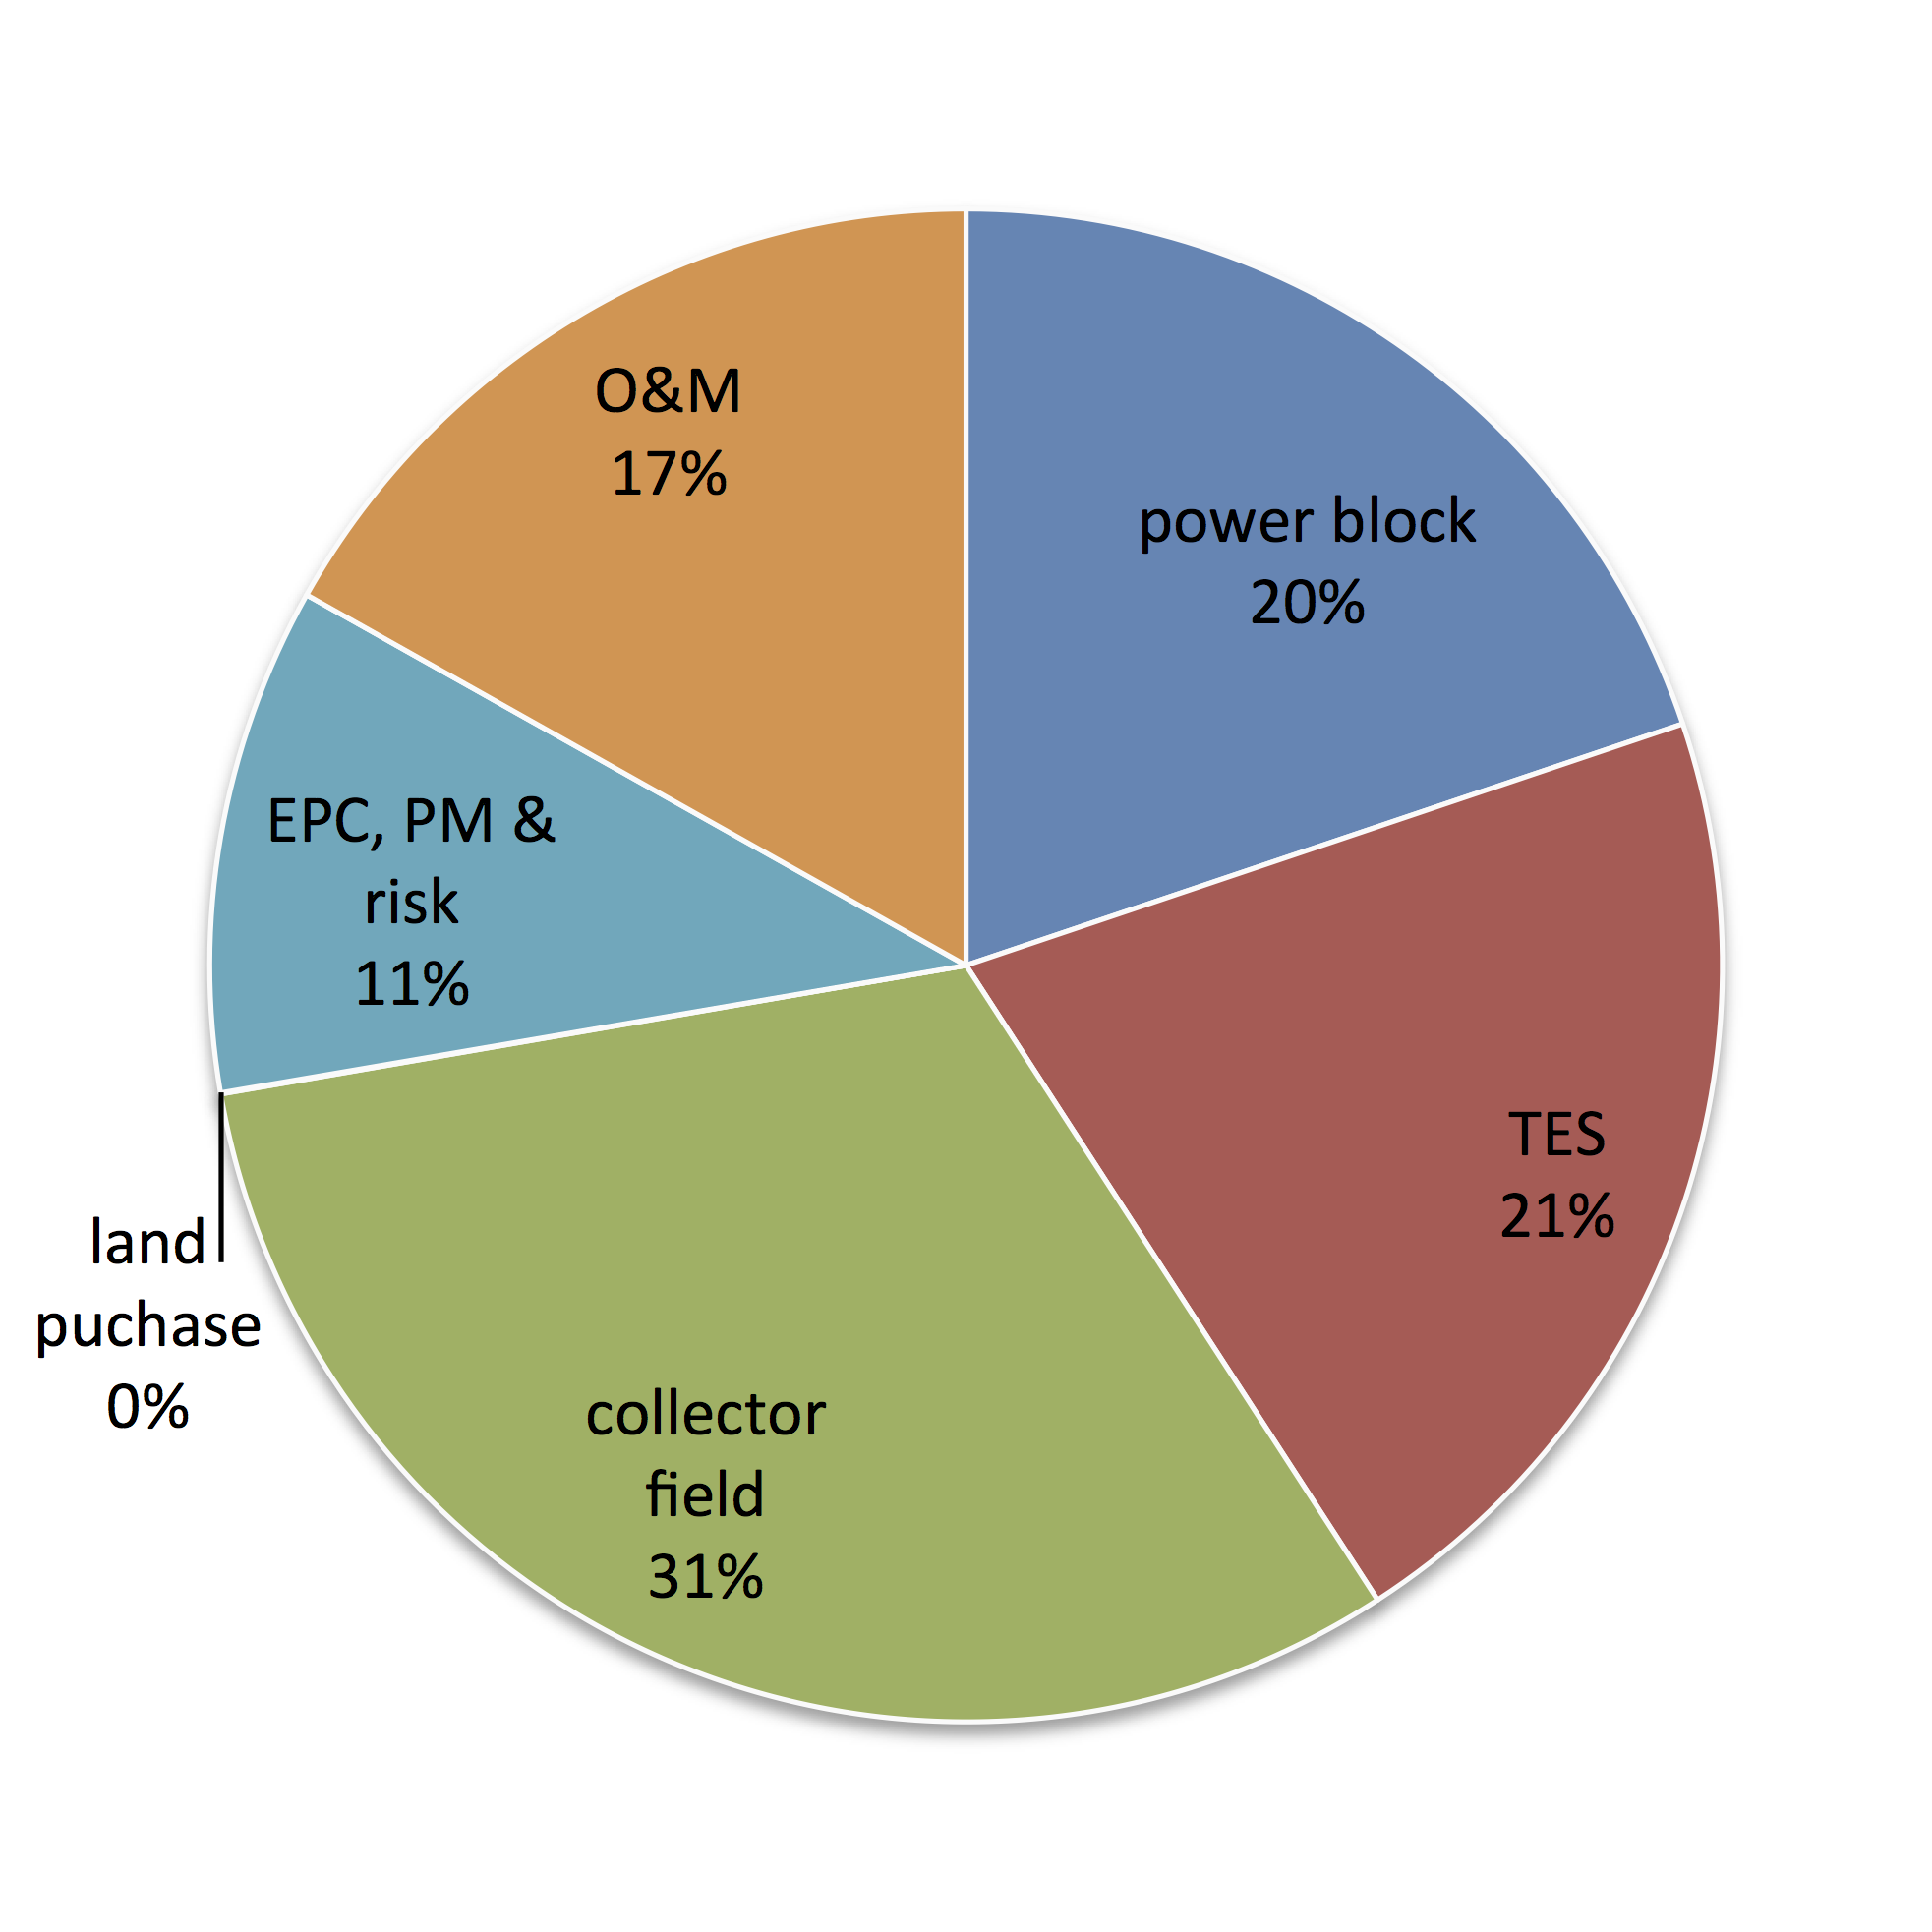
\includegraphics[width=1\textwidth]{FIG/PTC_LCOE_lowinvest_BreakDown}
                \caption{LCOE break-down for SM~2.0 and \SI{8}{h}~TES.}\label{PTC_LCOE_lowinvest_BreakDown}
        \end{subfigure}%
        ~
        \begin{subfigure}[b]{0.5\textwidth}
                \centering
                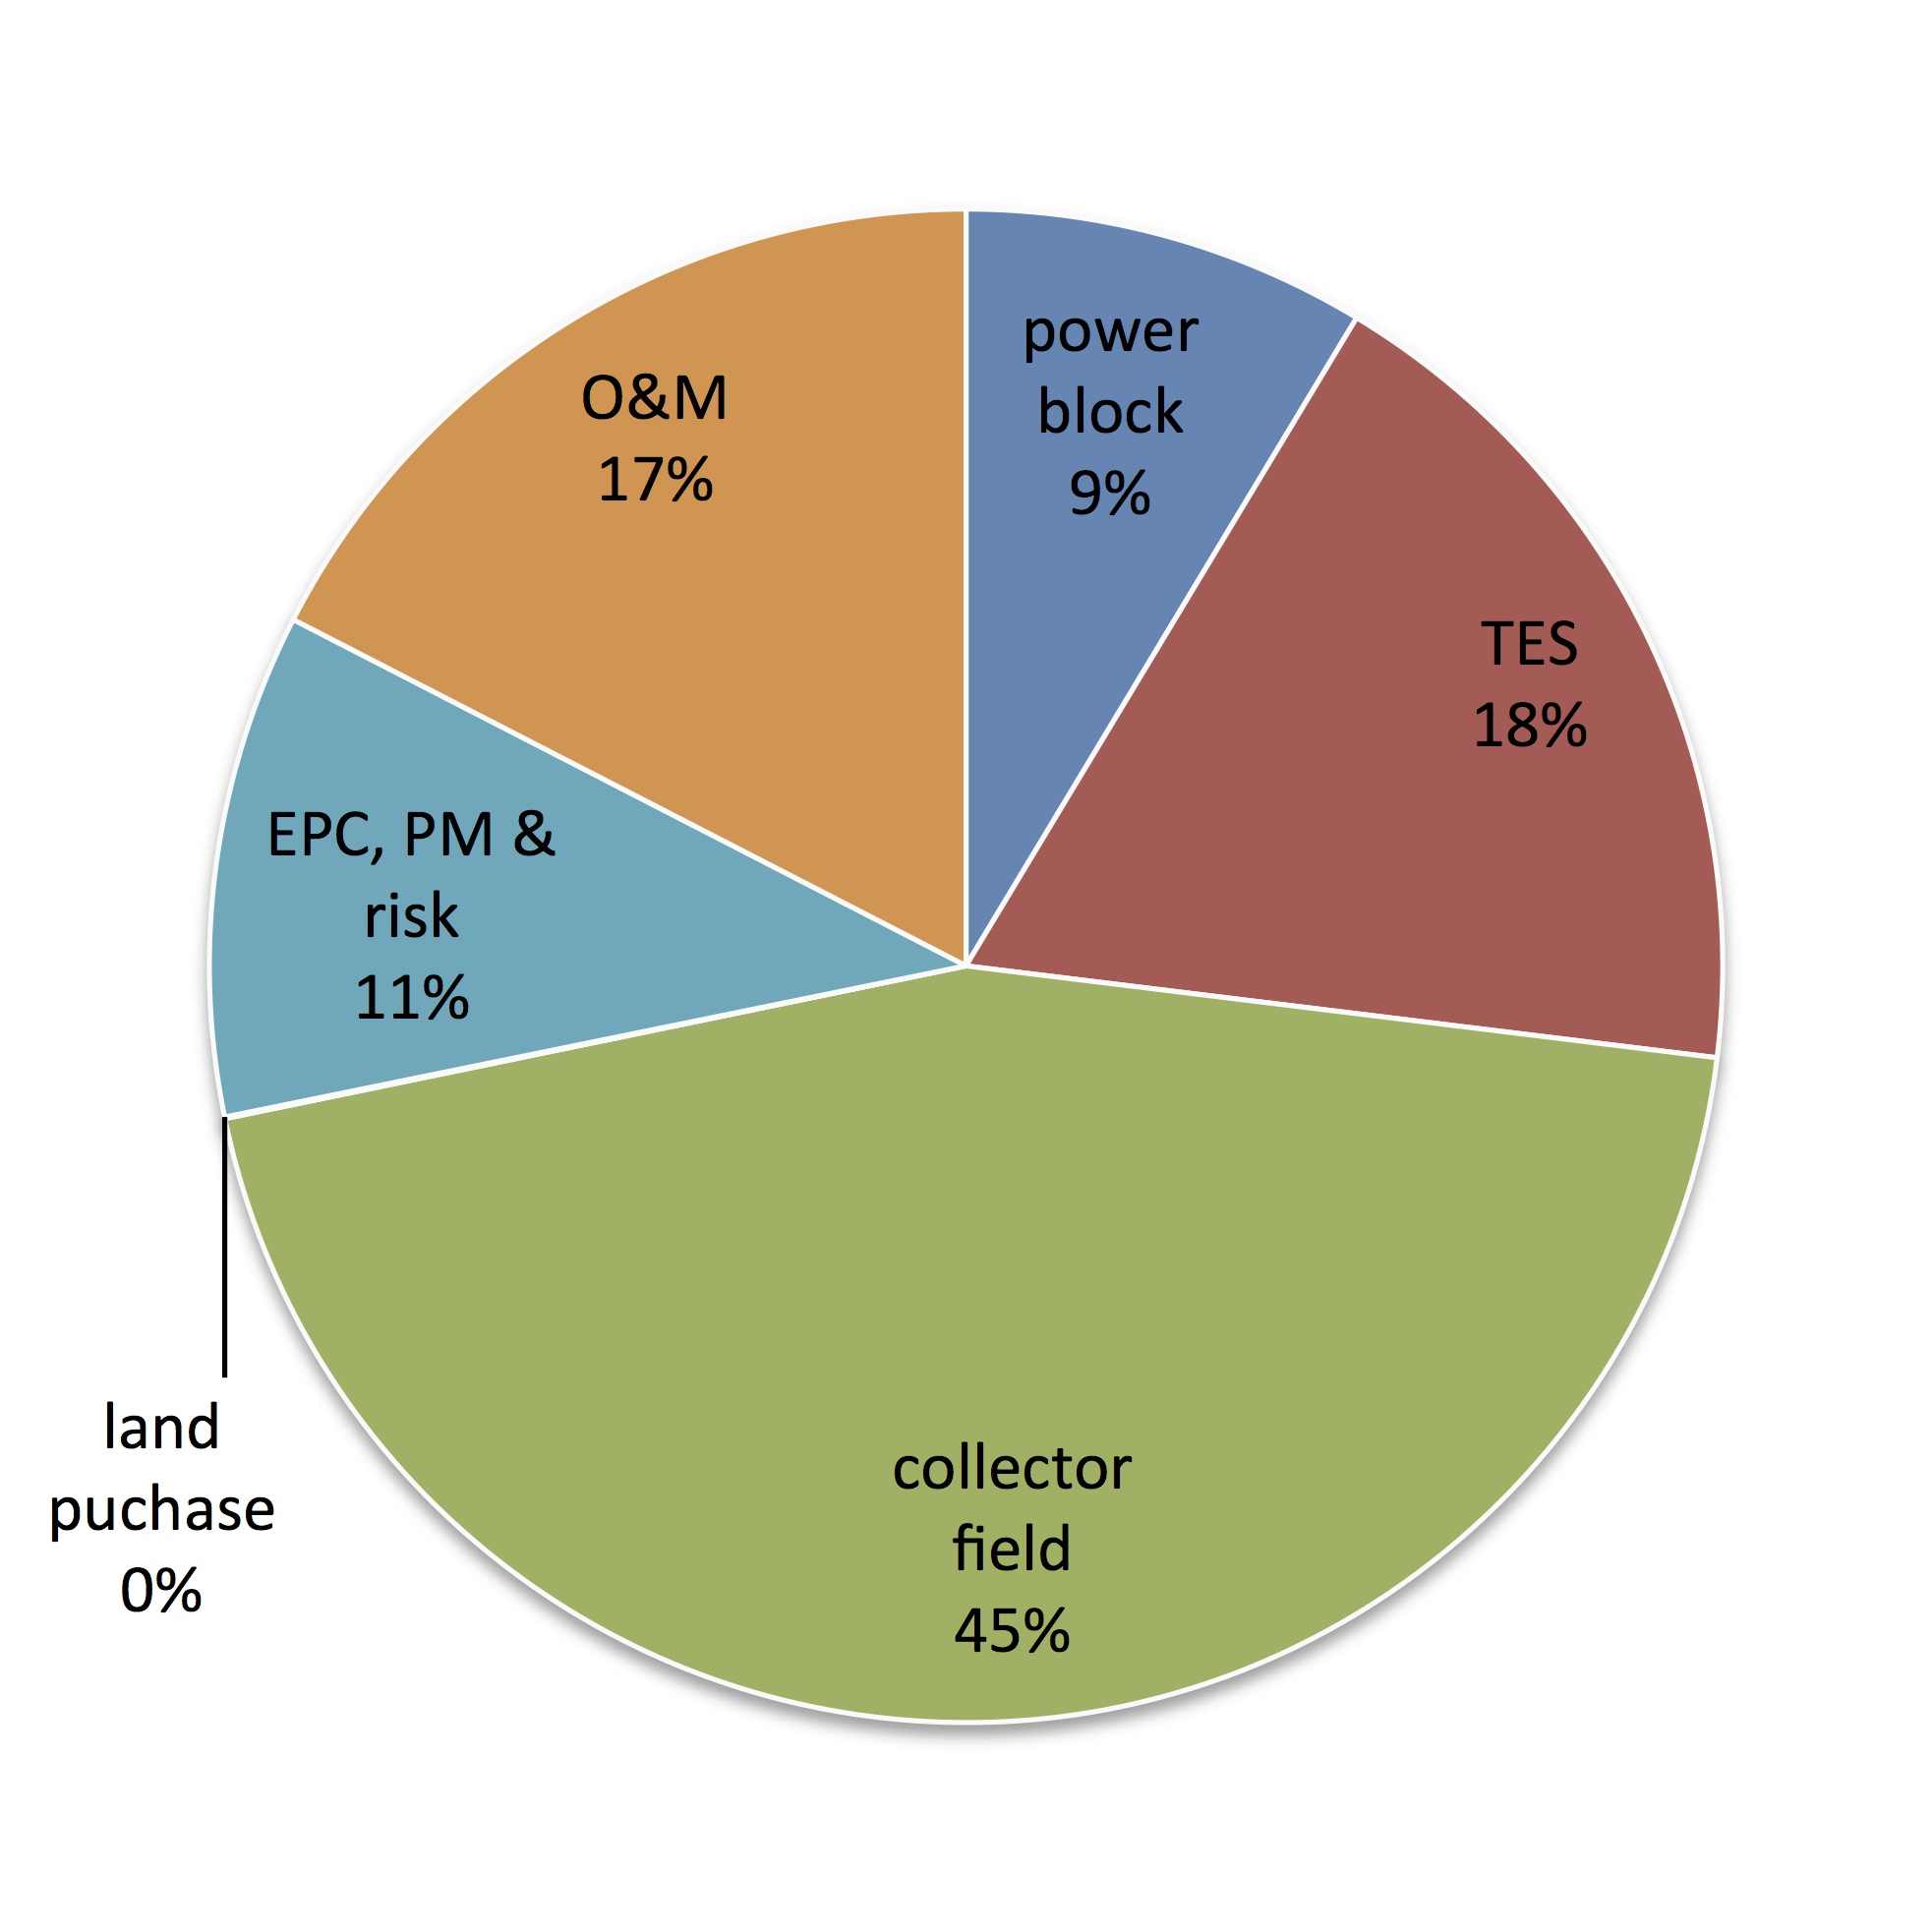
\includegraphics[width=1\textwidth]{FIG/PTC_LCOE_highinvest_BreakDown}
                \caption{LCOE break-down for SM~5.0 and \SI{16}{h}~TES.}\label{PTC_LCOE_highinvest_BreakDown}
        \end{subfigure}
        \caption[Break-down of selected PTC-LCOE calculation results.]{Break-down of selected PTC-LCOE calculation results.}\label{PTC_LCOE_BreakDown}
\end{figure}
\pagebreak